% !TeX program = xelatex
% Overleaf: choose XeLaTeX as the compiler.
\documentclass[11pt,a4paper,fontset=fandol]{ctexart}
\usepackage[margin=2.3cm]{geometry}
\usepackage{amsmath,amssymb}
\usepackage{enumitem}
\usepackage{tikz}
\usepackage{hyperref}
\hypersetup{colorlinks=true,linkcolor=blue,urlcolor=blue}
\setlength{\parindent}{0pt}
\setlength{\parskip}{0.5em}
\setlist[enumerate]{itemsep=0.25em,topsep=0.3em}
\providecommand{\tightlist}{\setlength{\itemsep}{0pt}\setlength{\parskip}{0pt}}
\setcounter{secnumdepth}{0}
\setcounter{tocdepth}{2}
\title{GRE Mathematics 错题与不确定题笔记}
\author{}
\date{}
\begin{document}
\maketitle
\tableofcontents
\clearpage

\section{每日晨读：群论、环的基础与复变留数}
\label{review:morning}
本节先于各套错题，供晨读。目标是看到题目就能识别适用条件，而不是只背公式；特别区分一般群与循环群、加法群与乘法群、极点阶数与留数。MathSub 的题面勘误见 \hyperref[ms:q52]{52题}、\hyperref[ms:q62]{62题}。

\subsection{群论与数论：英文、性质及条件}
\label{review:groups}
\textbf{基本词义。}group：群；abelian/commutative：交换的；closure：封闭性；identity：单位元；inverse：逆元；order of a group：群阶 $|G|$，即元素个数；order of an element：元素阶 $\operatorname{ord}(a)$，即使 $a^m=e$ 的最小正整数 $m$，不存在则为无限阶；cyclic：循环的；generator：生成元；subgroup：子群；proper subgroup：真子群 $H\ne G$；trivial subgroup：平凡子群 $\{e\}$；index：指数 $[G:H]$，即陪集个数；coprime/relatively prime：互素。元素本身的数值不等于它的阶。

\textbf{群与子群判别。}群运算封闭、满足结合律、有单位元且每个元素有逆元，不要求交换。非空子集 $H\subseteq G$ 是子群，当且仅当对所有 $x,y\in H$ 有 $xy^{-1}\in H$；加法记号下是 $x-y\in H$。有限非空子集若对乘法封闭，则自动为子群；无限子集不能这样推，例如正整数对加法封闭，却不是整数加法群的子群。

\textbf{元素阶与模运算。}若 $\operatorname{ord}(a)=n<\infty$，则
\begin{equation}
a^k=e\iff n\mid k,\qquad a^r=a^s\iff r\equiv s\pmod n,\qquad
\operatorname{ord}(a^k)=\frac{n}{\gcd(n,k)}.
\label{review:order-power}
\end{equation}
最后一个公式来自 $(a^k)^t=e\iff n\mid kt$，取满足条件的最小正整数 $t$。例如 $a$ 的阶为30，则 $a^{12}$ 的阶为5。逆元 $a^{-1}$ 与 $a$ 的阶相同。

\textbf{拉格朗日定理（Lagrange）。}有限群中
\begin{equation}
|G|=[G:H]|H|,\qquad |H|\mid|G|,\qquad \operatorname{ord}(a)\mid|G|,\qquad a^{|G|}=e.
\label{review:lagrange}
\end{equation}
方向不能反过来：$d\mid|G|$ 不保证存在 $d$ 阶子群，更不保证存在 $d$ 阶元素。见 \hyperref[ms:q38]{MathSub 38题}。

\textbf{循环群的子群。}若 $G=\langle a\rangle$、$|G|=n$，则每个子群都循环；对每个正因子 $d\mid n$，恰好有一个 $d$ 阶子群 $\langle a^{n/d}\rangle$。元素 $a^k$ 是生成元当且仅当 $\gcd(n,k)=1$，故生成元共有 $\varphi(n)$ 个。对每个 $d\mid n$，阶恰为 $d$ 的元素有 $\varphi(d)$ 个，而不是只有一个。若 $n=\prod p_j^{\alpha_j}$，子群总数为 $\prod(\alpha_j+1)$，其中
\[
\varphi(n)=n\prod_{p\mid n}(1-1/p).
\]
例如 $C_{12}$ 的6阶子群只有 $\langle a^2\rangle$ 一个，6阶元素却有 $a^2,a^{10}$ 两个。素数阶群必循环；$p^2$ 阶群必交换，但可能是 $C_{p^2}$ 或 $C_p\times C_p$，不一定循环。

\textbf{哪些子群一定存在？}柯西定理（Cauchy）：素数 $p\mid|G|$，则有 $p$ 阶元素，因而有 $p$ 阶子群。Sylow：若 $|G|=p^km$ 且 $p\nmid m$，则存在 $p^k$ 阶子群；这类子群个数 $n_p$ 满足 $n_p\mid m$、$n_p\equiv1\pmod p$，且 $n_p=1$ 当且仅当该 Sylow 子群正规。normal subgroup：正规子群，定义为对所有 $g\in G$ 有 $gHg^{-1}=H$；指数2的子群必正规。例如阶60保证有2、3、4、5阶子群，不能仅靠这些定理保证有6阶子群。

\textbf{直积与最小公倍数。}
\begin{equation}
\operatorname{ord}((a,b))=\operatorname{lcm}(\operatorname{ord}(a),\operatorname{ord}(b)),\qquad
C_m\times C_n\text{ 循环}\iff\gcd(m,n)=1.
\label{review:direct-product}
\end{equation}
群阶是分量群阶的乘积，单个元素的阶却是分量元素阶的 lcm。例如 $C_{22}\times C_{33}$ 群阶726，元素阶至多66，故不循环。多个有限循环群的直积循环，当且仅当各群阶两两互素。中国剩余定理给出互素时 $\mathbb Z_{mn}\cong\mathbb Z_m\times\mathbb Z_n$（也成立为环同构）。

\textbf{同一群中乘积 $ab$ 的阶。}若 $a,b$ 交换且阶分别为 $m,n$，则 $\operatorname{ord}(ab)\mid\operatorname{lcm}(m,n)$；若进一步 $\gcd(m,n)=1$，则阶为 $mn$。不互素时未必等于 lcm，例如 $b=a^{-1}$。不交换时不能套用：在 $S_3$ 中 $(12),(23)$ 都是2阶，乘积却是3阶。

\textbf{整数子群与贝祖等式。}$(\mathbb Z,+)$ 的子群全部是 $n\mathbb Z$（$n\ge0$）。对正整数 $m,n$，
\begin{equation}
\langle m,n\rangle=\gcd(m,n)\mathbb Z,\qquad
m\mathbb Z\cap n\mathbb Z=\operatorname{lcm}(m,n)\mathbb Z,\qquad
m\mathbb Z\subseteq n\mathbb Z\iff n\mid m.
\label{review:integer-subgroups}
\end{equation}
贝祖等式说 $\gcd(m,n)=um+vn$，其中 $u,v$ 为整数；所以真子群不能同时包含两个互素整数。数值越大，其倍数集合不一定包含另一集合，要用整除判断。

\textbf{有限循环群中的交与生成。}若 $H,K$ 是同一有限循环群的子群，阶分别为 $r,s$，则 $|H\cap K|=\gcd(r,s)$、$|\langle H\cup K\rangle|=\operatorname{lcm}(r,s)$。一般有限群只能保证共同生成子群的阶是 lcm 的倍数，不能保证等于 lcm。

\textbf{模 $n$ 加法群与乘法群不能混淆。}$(\mathbb Z_n,+)$ 有 $n$ 个元素，单位元是0，元素 $[a]$ 的阶为 $n/\gcd(a,n)$。$\mathbb Z_n^\times$ 则是所有可逆剩余类组成的乘法群，单位元是1，群阶为 $\varphi(n)$；$[a]$ 可逆当且仅当 $\gcd(a,n)=1$。乘法阶是最小的 $k>0$ 使 $a^k\equiv1\pmod n$，不能套加法阶公式。例如模7时2的乘法阶为3。对这个乘法群用拉格朗日定理得到欧拉定理 $a^{\varphi(n)}\equiv1\pmod n$（要求互素）；素数模数时得到费马小定理。

\textbf{同态。}homomorphism：保持运算的映射 $\phi(ab)=\phi(a)\phi(b)$；kernel：核 $\ker\phi=\{a:\phi(a)=e\}$，是正规子群；image：像 $\operatorname{im}\phi$，是目标群的子群。第一同构定理给出 $G/\ker\phi\cong\operatorname{im}\phi$；有限时 $|G|=|\ker\phi|\,|\operatorname{im}\phi|$。所以像的阶同时整除定义域群阶与目标群阶，两阶互素时任何同态都平凡。

\subsection{环：只补做题所需的基本定义}
\label{review:rings}
环（ring）的加法构成交换群，乘法结合，且满足左右分配律；乘法不一定交换，不同教材对是否要求单位元约定不同。此处涉及可逆元时使用含幺环，且通常 $1\ne0$。unity/multiplicative identity 是乘法单位元1；unit 却是\textbf{可逆元}，要求存在 $b$ 使 $ab=ba=1$，不是在问有几个单位元。zero divisor 是非零元 $a$，能与某个非零元相乘得到0（非交换时区分左右）；integral domain 是无零因子的非零交换含幺环；field 是每个非零元都可逆的非零交换含幺环；division ring 允许不交换。

双侧理想（two-sided ideal）$I$ 是加法子群，且对所有 $a\in I,r\in R$ 有 $ra,ar\in I$。理想一定含0，但不一定含1；若 $1\in I$，则 $r=r1\in I$，从而 $I=R$。例如 $2\mathbb Z$ 是 $\mathbb Z$ 的理想，不包含1。$\mathbb Z$ 的理想全为 $n\mathbb Z$。通常的理想乘积允许有限和：
\[
AB=\left\{\sum_{j=1}^m a_jb_j:a_j\in A,b_j\in B,m\ge1\right\},\qquad
AB\subseteq A\cap B\subseteq A+B.
\]
只允许单个乘积的集合未必是理想，参见 Practice 1 的50题；允许有限和的定义见 \hyperref[ms:q64]{MathSub 64题}。交换含幺环中，真理想 $I$ 极大当且仅当 $R/I$ 是域，素当且仅当 $R/I$ 是整环。域的理想只有零理想和全环。

\subsection{复变：解析性、柯西--黎曼方程与留数的原理}
\label{review:residues}
\textbf{英文与基本结论。}holomorphic：全纯，在开区域内处处复可微；analytic：解析，局部可展开为收敛幂级数，一元复分析中二者等价；entire：整函数，在整个 $\mathbb C$ 上全纯；pole：极点；residue：留数；singularity：奇点；counterclockwise：逆时针，取正方向。写 $f=u+iv$，解析函数满足 Cauchy--Riemann 方程
\begin{equation}
u_x=v_y,\qquad u_y=-v_x.
\label{review:cr}
\end{equation}
反向使用时，常用充分条件是这些偏导数在邻域存在且连续，并在该点满足方程；仅在一点形式满足方程未必足够。连通开区域上的解析函数若全取实值或模长恒定，必常值；仅在一条实轴或区域边界上成立则不足。非恒定解析函数为开映射；有界整函数必常值（Liouville）；局部解析函数在 $a$ 的 Taylor 系数为 $f^{(n)}(a)/n!$。

\textbf{Taylor 与 Laurent。}若中心 $a$ 也解析，展开只有非负整数次幂。若仅在穿孔圆盘 $0<|z-a|<R$ 解析，则可写
\begin{equation}
f(z)=\sum_{n=-\infty}^{\infty}c_n(z-a)^n,\qquad \operatorname{Res}(f,a)=c_{-1}.
\label{review:laurent}
\end{equation}
负次幂部分称主部：无非零负次项时中心可解析延拓；有限个非零负次项、最低次为 $-m$ 时为 $m$ 阶极点；无穷多个非零负次项时为本性奇点。必须在中心附近的穿孔圆盘判断，不能用远离中心的环域展开误判中心。例如 $1/(1-z)$ 在 $|z|<1$ 展开为 $\sum_{n\ge0}z^n$，在 $|z|>1$ 展开为 $-\sum_{n\ge1}z^{-n}$；后者不能用于判断0的奇点类型。

\textbf{为什么只看负一次项？}沿 $z=a+re^{it}$、$0\le t\le2\pi$，
\[
\oint_{|z-a|=r}(z-a)^n\,dz=ir^{n+1}\int_0^{2\pi}e^{i(n+1)t}\,dt
=\begin{cases}2\pi i,&n=-1,\\0,&n\ne-1,\end{cases}
\]
其中 $n$ 是整数。逐项积分时只有 $c_{-1}/(z-a)$ 留下。因此逆时针简单闭曲线 $C$ 内只有有限个孤立奇点、曲线上无奇点且其他位置解析时，
\begin{equation}
\oint_C f(z)\,dz=2\pi i\sum_{a\text{ 在 }C\text{ 内}}\operatorname{Res}(f,a).
\label{review:residue-theorem}
\end{equation}
原理是挖去奇点周围小圆，在剩余全纯区域应用柯西积分定理，把大边界积分变成各小圆积分之和。顺时针反号；前面若已有 $1/(2\pi i)$，答案直接为留数和；奇点在路径上不能直接套用。

\textbf{简单极点：为什么要除以分母导数？}设 $f=P/Q$，$Q(a)=0$、$Q'(a)\ne0$ 且 $P(a)\ne0$。把分母写成
\[
Q(z)=(z-a)H(z),\qquad H(a)=Q'(a).
\]
于是 $f(z)=[P(z)/H(z)]/(z-a)$，括号内解析，其常数项为 $P(a)/Q'(a)$。所以
\begin{equation}
\operatorname{Res}(P/Q,a)=\frac{P(a)}{Q'(a)}
=\lim_{z\to a}(z-a)f(z).
\label{review:simple-residue}
\end{equation}
例如 $3/(2z-2)=(3/2)/(z-1)$，留数为 $3/2$；不是令 $z-a=1$，而是提取负一次项系数。$\sin z$ 在 $\pi$ 附近一阶项为 $-(z-\pi)$，所以 $3/\sin z$ 在 $\pi$ 的留数为 $-3$。分子分母同时为零时先约分，可能降阶或成为可去奇点。

\textbf{高阶极点：求导只是提取同一个系数。}若 $f(z)=h(z)/(z-a)^m$，$h$ 在 $a$ 附近解析，则
\begin{equation}
\operatorname{Res}(f,a)=\frac{h^{(m-1)}(a)}{(m-1)!}.
\label{review:higher-residue}
\end{equation}
若 $h(a)\ne0$，它确实是 $m$ 阶极点；即使 $h(a)=0$，此系数公式仍成立，但实际阶数可能下降。原因是 $h$ 的 Taylor 展开中 $(m-1)$ 次项除以 $(z-a)^m$ 后，恰变成负一次项。二阶求 $h'(a)$，三阶求 $h''(a)/2!$，四阶求 $h'''(a)/3!$。若分母还有其他因子，必须并入 $h$ 整体求导，例如 $e^z/[(z-a)^4(z-b)]$ 在 $a\ne b$ 处应对 $h=e^z/(z-b)$ 求三阶导，不能只对分子 $e^z$ 求导。

\textbf{最容易混淆的两式。}常数分子 $e/(z-1)^2$ 已经只有负二次项，留数0；但
\[
\frac{e^z}{(z-1)^2}
=\frac{e[1+(z-1)+(z-1)^2/2+\cdots]}{(z-1)^2}
=\frac e{(z-1)^2}+\frac e{z-1}+\frac e2+\cdots,
\]
留数为 $e$。不是负二次项贡献了积分，而是分子的变化产生了负一次项。极点阶数看最负次项；积分只看负一次项；不能看见平方分母就宣布积分0。

\textbf{常用算例。}以下圆均逆时针，均无路径上极点：
\[
\begin{array}{c|c|c}
f(z),\ C&\text{内部留数}&\oint_Cf(z)\,dz\\\hline
1/(z^2+1),\ |z|=2&1/(2i),\ -1/(2i)&0\\
1/(z^2+1),\ |z-i|=1&1/(2i)&\pi\\
(z+2)/(z^2+1),\ |z|=2&1/2-i,\ 1/2+i&2\pi i\\
(z+1)/(e^z-2),\ |z|=1&(1+\ln2)/2&\pi i(1+\ln2)\\
e^z/(z-1)^2,\ |z|=2&e&2\pi i e
\end{array}
\]
第四例的分母零点是 $\ln2+2k\pi i$，圆内只有 $\ln2$。三个候选极点的例子：$(z+2)/[(z^2+1)(z-3)]$ 沿 $|z|=2$，只算 $\pm i$，留数分别为 $-1/4\pm i/4$，积分 $-\pi i$。混合阶数例子：$(z+1)/[(z-1)^2(z+2)]$ 在1的留数是 $\left[(z+1)/(z+2)\right]'_{z=1}=1/9$，在 $-2$ 是 $-1/9$；沿 $|z|=3$ 积分0，只包围1则为 $2\pi i/9$。

\textbf{收敛半径的快速联系。}有理函数先消去可去因子，围绕 $a$ 的 Taylor 收敛半径是到最近复极点的距离；不是只找实数奇点。例如 $2z/(z^2+1)$ 围绕 $-1$ 展开，最近极点 $\pm i$ 距离均为 $\sqrt2$，见 \hyperref[ms:q31]{31题}。

\textbf{晨读检查。}群论先查一般群还是循环群、阶是元素阶还是群阶、运算是加法还是乘法；环题分清 unit 与 unity、理想是否含1；留数题先查展开中心、圆内奇点、是否消去、极点阶数，最后取负一次项系数并检查方向和 $2\pi i$。可回看 \hyperref[review:order-power]{幂的阶}、\hyperref[review:direct-product]{直积公式}、\hyperref[review:simple-residue]{简单极点}、\hyperref[review:higher-residue]{高阶极点}。
\clearpage
\hypertarget{gre-mathematics-ux9519ux9898ux4e0eux4e0dux786eux5b9aux9898practice-1}{%
\section{GRE Mathematics 错题与不确定题：Practice
1}\label{gre-mathematics-ux9519ux9898ux4e0eux4e0dux786eux5b9aux9898practice-1}}

本次记录 10
道错题：24、27、43、44、50、53、60、62、64、65；另收录答对但不确定的
36、37。题号和选项对应 Practice
1。错因依据作答者自述；错题不自动等于知识漏洞，猜对也不等于掌握。

\hypertarget{ux9f50ux6b21ux65b9ux7a0bux7ec4ux7684ux89e3ux7a7aux95f4e}{%
\subsection{24.
齐次方程组的解空间：E}\label{ux9f50ux6b21ux65b9ux7a0bux7ec4ux7684ux89e3ux7a7aux95f4e}}

\textbf{原题（Original problem）}\par
Consider the system of linear equations
\[\begin{aligned}w+3x+2y+2z&=0,\\ w+4x+y&=0,\\ 3w+5x+10y+14z&=0,\\ 2w+5x+5y+6z&=0.\end{aligned}\]
with solutions of the form $(w,x,y,z)$, where $w$, $x$, $y$, and $z$ are real. Which of the following statements is FALSE?
\begin{enumerate}[label=(\Alph*)]
\item The system is consistent. \item The system has infinitely many solutions. \item The sum of any two solutions is a solution. \item $(-5,1,1,0)$ is a solution. \item Every solution is a scalar multiple of $(-5,1,1,0)$.
\end{enumerate}
\textbf{词语：}consistent：有解（has at least one solution）；scalar multiple：标量倍数；FALSE：错误的。

\textbf{解答与分析}\par


\textbf{错因：}误解 consistent，且未验证解空间维数。consistent
意为至少有一个解；齐次方程组一定有零解，因此必 consistent。

第二式给 \(w=-4x-y\)，代入第一式得 \(x=y+2z\)，因此

\[ (w,x,y,z)=y(-5,1,1,0)+z(-8,2,0,1). \]

另外两式也满足。两个向量线性无关，所以解空间维数为
2，并非所有解都是第一个向量的倍数，E 错。A 正确；B 有无穷多解；C
因线性性成立；D 可直接代入。一般而言齐次系统 \(Ax=0\)
的解构成子空间，维数为未知数个数减去
\(\operatorname{rank}A\)；非齐次系统有解才称
consistent，其解集一般是一个仿射空间。

\hypertarget{ux590dux6570ux7684ux5e45ux89d2ux4e0eux6a21d}{%
\subsection{27.
复数的幅角与模：D}\label{ux590dux6570ux7684ux5e45ux89d2ux4e0eux6a21d}}

\textbf{原题（Original problem）}\par
$(1+i)^{10}=$
\begin{enumerate}[label=(\Alph*),nosep]
\item $1$ \item $i$ \item $32$ \item $32i$ \item $32(i+1)$
\end{enumerate}
\textbf{词语：}modulus：复数的模；argument：复数的幅角。

\textbf{解答与分析}\par


\textbf{错因：}只考虑幅角，漏掉模长。

\[ (1+i)^{10}=\bigl(\sqrt2\,e^{i\pi/4}\bigr)^{10}=32e^{5\pi i/2}=32i. \]

也可用 \((1+i)^2=2i\)，得到
\((2i)^5=32i\)。复数乘方时，模取幂、幅角乘指数；两者缺一不可。

\hypertarget{ux5185ux90e8ux95edux5305ux548cux8fdeux901acux7b54ux5bf9ux4f46ux4e0dux786eux5b9a}{%
\subsection{36.
内部、闭包和连通：C（答对但不确定）}\label{ux5185ux90e8ux95edux5305ux548cux8fdeux901acux7b54ux5bf9ux4f46ux4e0dux786eux5b9a}}

\textbf{原题（Original problem）}\par
Suppose $S$ is a nonempty subset of $\mathbb R$. Which of the following is necessarily true?
\begin{enumerate}[label=(\Alph*)]
\item For each $s,t\in S$, there exists a continuous function $f$ mapping $[0,1]$ into $S$ with $f(0)=s$ and $f(1)=t$.
\item For each $u\notin S$, there exists an open subset $U$ of $\mathbb R$ such that $u\in U$ and $U\cap S=\varnothing$.
\item $\{v\in S:\text{there exists an open subset }V\text{ of }\mathbb R\text{ with }v\in V\subseteq S\}$ is an open subset of $\mathbb R$.
\item $\{w\notin S:\text{there exists an open subset }W\text{ of }\mathbb R\text{ with }w\in W\text{ and }W\cap S=\varnothing\}$ is a closed subset of $\mathbb R$.
\item $S$ is the intersection of all closed subsets of $\mathbb R$ that contain $S$.
\end{enumerate}
\textbf{词语：}necessarily true：必然成立；open/closed subset：开/闭子集；intersection：交集。

\textbf{解答与分析}\par


C 所述集合恰是内部 \(S^\circ\)：所有存在开邻域包含于 \(S\)
的点。它是所有包含于 \(S\) 的开集之并，因而开。

\begin{itemize}
\tightlist
\item
  A 要求任意两点之间有包含于 \(S\) 的连续路径；取 \(S=\{0,1\}\)
  即不成立，因为连续函数在区间上的像是连通的。
\item
  B 要求每个不属于 \(S\) 的点有不碰 \(S\) 的开邻域；取
  \(S=(0,1)\)、\(u=0\)，不成立。
\item
  D 所述集合是 \(\mathbb R\setminus\overline S\)，总是开集，不一定闭。取
  \(S=[0,1]\)。
\item
  E 中所有包含 \(S\) 的闭集之交是闭包 \(\overline S\)，不一定是
  \(S\)；取 \(S=(0,1)\)。
\end{itemize}

\textbf{速记：}内部是最大开子集，闭包是最小闭超集，边界为
\(\overline S\setminus S^\circ\)。集合开不代表不闭，闭不代表不开。

\hypertarget{ux5e42ux7b49ux53d8ux6362cux7b54ux5bf9ux4f46ux4e0dux786eux5b9a}{%
\subsection{37.
幂等变换：C（答对但不确定）}\label{ux5e42ux7b49ux53d8ux6362cux7b54ux5bf9ux4f46ux4e0dux786eux5b9a}}

\textbf{原题（Original problem）}\par
Let $V$ be a finite-dimensional real vector space and let $P$ be a linear transformation of $V$ such that $P^2=P$. Which of the following must be true?
\begin{enumerate}[label=\Roman*.]
\item $P$ is invertible. \item $P$ is diagonalizable. \item $P$ is either the identity transformation or the zero transformation.
\end{enumerate}
(A) None \quad (B) I only \quad (C) II only \quad (D) III only \quad (E) II and III.

\textbf{词语：}invertible：可逆；diagonalizable：可对角化；identity transformation：恒等变换。

\textbf{解答与分析}\par


\textbf{基本概念。}像空间与核空间分别定义为
\[
\operatorname{im}P=\{P(v):v\in V\},\qquad
\ker P=\{v\in V:P(v)=0\}.
\]

\textbf{第一步：像空间中的向量经过 \(P\) 后不变。}任取 \(u\in\operatorname{im}P\)，由定义存在 \(v\in V\) 使 \(u=P(v)\)。因此
\[
P(u)=P(P(v))=P^2(v)=P(v)=u.
\]
所以 \(P\) 在像空间上是恒等变换；其中的每个非零向量都是特征值 \(1\) 的特征向量。

\textbf{第二步：核空间中的向量经过 \(P\) 后变为零。}若 \(w\in\ker P\)，则按核的定义 \(P(w)=0\)。因此核空间中的每个非零向量都是特征值 \(0\) 的特征向量。

\textbf{第三步：证明 \(V=\operatorname{im}P\oplus\ker P\)。}任取 \(v\in V\)，写成
\[
v=P(v)+\bigl(v-P(v)\bigr).
\]
第一项 \(P(v)\in\operatorname{im}P\)。对第二项作用 \(P\)，由线性性与 \(P^2=P\)，
\[
P\bigl(v-P(v)\bigr)=P(v)-P^2(v)=0,
\]
故 \(v-P(v)\in\ker P\)。这证明每个向量都是像空间中的向量与核空间中的向量之和，即 \(V=\operatorname{im}P+\ker P\)。

这个分解还是唯一的：若 \(u\in\operatorname{im}P\cap\ker P\)，由第一步有 \(P(u)=u\)，由核的定义又有 \(P(u)=0\)，故 \(u=0\)。因此两个子空间交集仅含零向量，得到直和
\[
V=\operatorname{im}P\oplus\ker P.
\]

\textbf{第四步：选基并写出矩阵。}取像空间的一组基 \(u_1,\ldots,u_r\)，以及核空间的一组基 \(w_1,\ldots,w_s\)。上述直和分解保证
\[
\mathcal B=(u_1,\ldots,u_r,w_1,\ldots,w_s)
\]
是 \(V\) 的一组基。对这些基向量，
\[
P(u_i)=u_i\quad(1\le i\le r),\qquad P(w_j)=0\quad(1\le j\le s).
\]
矩阵的每一列是相应基向量的像在基 \(\mathcal B\) 下的坐标，因此
\[
[P]_{\mathcal B}=
\begin{pmatrix}I_r&0\\0&0\end{pmatrix}
=\operatorname{diag}(\underbrace{1,\ldots,1}_{r},
\underbrace{0,\ldots,0}_{s}).
\]
这是一个对角矩阵。于是 \(P\) 有一组由特征向量组成的基，故 \(P\) 可对角化，II 成立。若像空间或核空间是零空间，则相应的一组基为空，上述结论仍成立。

\textbf{具体例子。}在 \(\mathbb R^2\) 上令 \(P(x,y)=(x,0)\)。则 \(P^2=P\)，像空间为 \(x\) 轴 \(\operatorname{span}\{(1,0)\}\)，核空间为 \(y\) 轴 \(\operatorname{span}\{(0,1)\}\)。在由这两个向量组成的基下，矩阵为
\[
\begin{pmatrix}1&0\\0&0\end{pmatrix}.
\]
I 不一定成立：零变换在非零空间上不可逆。III 不一定成立：这个例子既非恒等变换也非零变换。因此答案为 C。

\textbf{易错点。}仅证明特征值属于 \(\{0,1\}\) 本身不足以证明可对角化；还需要证明存在足够多的线性无关特征向量。上述直和分解给出了完整特征向量基。也可使用最小多项式整除无重根多项式 \(t(t-1)\) 来证明。

\hypertarget{ux53c2ux6570ux66f2ux7ebfux4e8cux9636ux5bfcux6570a}{%
\subsection{43.
参数曲线二阶导数：A}\label{ux53c2ux6570ux66f2ux7ebfux4e8cux9636ux5bfcux6570a}}

\textbf{原题（Original problem）}\par
A curve in the $xy$-plane is given parametrically by
\[x=t^2+2t,\qquad y=3t^4+4t^3\]
for all $t>0$. The value of $d^2y/dx^2$ at the point $(8,80)$ is

(A) $4$ \quad (B) $24$ \quad (C) $32$ \quad (D) $96$ \quad (E) $192$.

\textbf{词语：}given parametrically：以参数方程给出；second derivative：二阶导数。

\textbf{解答与分析}\par


\textbf{错因：}求解过快。\(x=t^2+2t,\ y=3t^4+4t^3\)，由 \(t>0\) 和
\(x=8\) 得 \(t=2\)。先求

\[\frac{dy}{dx}=\frac{12t^3+12t^2}{2t+2}=6t^2,\qquad \frac{d^2y}{dx^2}=\frac{d(6t^2)/dt}{dx/dt}=\frac{12t}{2t+2}.\]

代入 \(t=2\) 得 4。每次对 \(x\) 求导，都要除以 \(dx/dt\)；不是直接对
\(t\) 求两次导数。

\hypertarget{ux4e00ux9636ux5faeux5206ux65b9ux7a0bb}{%
\subsection{44.
一阶微分方程：B}\label{ux4e00ux9636ux5faeux5206ux65b9ux7a0bb}}

\textbf{原题（Original problem）}\par
\[y'+xy=x,\qquad y(0)=-1.\]
If $y$ is a real-valued function defined on the real line and satisfying the initial value problem above, then $\displaystyle\lim_{x\to-\infty}y(x)=$

(A) $0$ \quad (B) $1$ \quad (C) $-1$ \quad (D) $\infty$ \quad (E) $-\infty$.

\textbf{词语：}initial value problem：初值问题；real-valued：取实值的；satisfying：满足。

\textbf{解答与分析}\par


\textbf{错因：}符号未代回原式核验。\(y'+xy=x,\ y(0)=-1\)。令
\(u=y-1\)，则 \(u'=-xu\)，所以

\[y=1+Ce^{-x^2/2}=1-2e^{-x^2/2},\qquad \lim_{x\to-\infty}y(x)=1.\]

检验：\(y'=2xe^{-x^2/2}\)，故 \(y'+xy=x\)，且 \(y(0)=-1\)。分离变量时
\(\int -x\,dx=-x^2/2\)；绝对值和任意常数应处理正确。

\hypertarget{ux7406ux60f3ux7684ux548cux9010ux9879ux4e58ux79efux4e0eux4ea4d}{%
\subsection{50.
理想的和、逐项乘积与交：D}\label{ux7406ux60f3ux7684ux548cux9010ux9879ux4e58ux79efux4e0eux4ea4d}}

\textbf{原题（Original problem）}\par
Let $R$ be a ring and let $U$ and $V$ be (two-sided) ideals of $R$. Which of the following must also be ideals of $R$?
\begin{enumerate}[label=\Roman*.]
\item $U+V=\{u+v:u\in U\text{ and }v\in V\}$.
\item $U\cdot V=\{uv:u\in U\text{ and }v\in V\}$.
\item $U\cap V$.
\end{enumerate}
(A) II only \quad (B) III only \quad (C) I and II only \quad (D) I and III only \quad (E) I, II, and III.

\textbf{词语：}ring：环；(two-sided) ideal：（双侧）理想；must also be：也必定是。注意 II 在题目中明确指单个乘积的集合。

\textbf{解答与分析}\par


\textbf{错因：}理想的闭合条件及理想乘积的定义不熟。双侧理想 \(I\)
是加法子群，且对 \(r\in R,a\in I\)，有 \(ra,ar\in I\)。

I：\(U+V=\{u+v\}\) 是理想；加法与左右乘吸收分别由 \(U,V\)
的性质得到。III：\(U\cap V\) 是理想，因为相关运算同时留在 \(U\) 和
\(V\)。

II：题目只允许\textbf{单个乘积}构成的集合
\(\{uv:u\in U,v\in V\}\)，不一定对加法封闭。具体取
\(R=\mathbb R[x,y]\)、\(U=V=(x,y)\)。\(x^2,y^2\) 都是单个乘积，但
\(x^2+y^2\) 不是两个属于 \((x,y)\)
的多项式的乘积：若能分解，两个因子的最低非零齐次部分均为实线性式，它们的乘积应为
\(x^2+y^2\)，然而后者不能分解为两个实线性式。故 II 不成立。

\textbf{相关高频知识：}

\begin{enumerate}
\def\labelenumi{\arabic{enumi}.}
\tightlist
\item
  通常的理想乘积 \(UV\) 定义为有限和
  \(\{\sum_{i=1}^m u_iv_i\}\)，不是单个乘积集合；它总是双侧理想，且
  \(UV\subseteq U\cap V\)。理想的并一般不是理想；两个理想的并是理想当且仅当其中一个包含另一个。
\item
  环同态的核是理想；商环 \(R/I\) 需要 \(I\)
  是双侧理想。交换含幺环中，真理想 \(I\) 极大当且仅当 \(R/I\)
  是域；\(I\) 素当且仅当 \(R/I\) 是整环。域的理想只有 \(\{0\}\)
  和整个域。
\item
  \(\mathbb Z\) 的每个理想都是
  \(n\mathbb Z\)；\(a\mathbb Z+b\mathbb Z=\gcd(a,b)\mathbb Z\)，交为
  \(\operatorname{lcm}(a,b)\mathbb Z\)。\(\mathbb Z/n\mathbb Z\)
  是域当且仅当 \(n\) 为素数。
\item
  群同态的核是正规子群；有限群中元素的阶整除群的阶（拉格朗日定理），但阶整除不意味着一定存在该阶元素。循环群的子群均循环；阶为
  \(n\) 的循环群中 \(g^k\) 的阶为 \(n/\gcd(n,k)\)。
\end{enumerate}

\hypertarget{ux53d8ux4e0aux9650ux79efux5206ux4e0eux5149ux6ed1ux6027a}{%
\subsection{53.
变上限积分与光滑性：A}\label{ux53d8ux4e0aux9650ux79efux5206ux4e0eux5149ux6ed1ux6027a}}

\textbf{原题（Original problem）}\par
Let $f$ and $g$ be functions of a real variable such that $g(x)=\int_0^x f(y)(y-x)\,dy$ for all $x$. If $g$ is three times continuously differentiable, what is the greatest integer $n$ for which $f$ must be $n$ times continuously differentiable?

(A) $1$ \quad (B) $2$ \quad (C) $3$ \quad (D) $4$ \quad (E) $5$.

\textbf{词语：}continuously differentiable：连续可微；greatest integer：最大整数；must be：必然满足。

\textbf{解答与分析}\par


题设 \(g(x)=\int_0^x f(y)(y-x)\,dy\)，给定 \(g\in C^3\)，求必须有
\(f\in C^n\) 的最大 \(n\)。解题时要注意方向：从 \(g\)
的正则性\textbf{反推} \(f\)。

在通常的连续被积函数假设下，莱布尼茨公式给出

\[g'(x)=-\int_0^x f(y)\,dy,\qquad g''(x)=-f(x),\qquad g'''(x)=-f'(x).\]

因此 \(f=-g''\in C^1\)。不一定是 \(C^2\)：取 \(f(x)=|x|^{3/2}\)，它属于
\(C^1\) 但在 0 不属于 \(C^2\)；由上式构造的 \(g\) 属于
\(C^3\)，故不能保证更多。

关于题设的细节：原题未明确写 \(f\) 连续。若只按通常 Riemann
积分理解，改变 \(f\) 在单个点的值不改变任何积分，却可破坏 \(f\)
的连续性；于是严格字面表述有缺口，A 需要补充 \(f\) 连续等假设。若按广义
Lebesgue 积分，更只能先得到几乎处处的结论。ETS 预期答案 A
基于通常的连续性假设，不应把这一隐含条件忽略。

你的直觉抓住了变上限积分带来的求导关系；这里具体是两次求导后恢复
\(-f\)，所以 \(g\) 的三次连续可微对应 \(f\) 的一次连续可微。

\hypertarget{ux91cfux8bcdux548cux65e0ux7a77ux8fdcux5904ux6781ux9650d}{%
\subsection{60.
量词和无穷远处极限：D}\label{ux91cfux8bcdux548cux65e0ux7a77ux8fdcux5904ux6781ux9650d}}

\textbf{原题（Original problem）}\par
A real-valued function $f$ defined on $\mathbb R$ has the following property.

For every positive number $\epsilon$, there exists a positive number $\delta$ such that $|f(x)-f(1)|\ge\epsilon$ whenever $|x-1|\ge\delta$.

This property is equivalent to which of the following statements about $f$?
\begin{enumerate}[label=(\Alph*)]
\item $f$ is continuous at $x=1$. \item $f$ is discontinuous at $x=1$. \item $f$ is unbounded. \item $\displaystyle\lim_{|x|\to\infty}|f(x)|=\infty$. \item $\displaystyle\int_0^\infty |f(x)|\,dx=\infty$.
\end{enumerate}
\textbf{词语：}whenever：只要；equivalent to：等价于；unbounded：无界。

\textbf{解答与分析}\par


题设是对每个 \(\varepsilon>0\)，存在 \(\delta>0\)，只要
\textbf{\(|x-1|\ge\delta\)}，就有
\textbf{\(|f(x)-f(1)|\ge\varepsilon\)}。它控制的是远离 1
的点，输出也远离 \(f(1)\)，不是连续性。连续性要求
\(|x-1|<\delta\Rightarrow|f(x)-f(1)|<\varepsilon\)。

令 \(c=f(1)\)。题设等价于 \(|f(x)-c|\to\infty\)，当
\(|x|\to\infty\)：因为 \(|x|\) 与 \(|x-1|\) 同时趋向无穷。再由

\[\bigl||f(x)|-|f(x)-c|\bigr|\le |c|\]

可知它等价于 \(|f(x)|\to\infty\)，即 D。形式上，如要证明 D，由题设选阈值
\(M+|c|+1\)，即可得到 \(|f(x)|>M\)；反向同理。

A 不等价：\(f(x)=x\)
连续且满足题设，但常数函数也连续，却不满足题设；另外令
\(f(1)=0\)、\(f(x)=x\)（\(x\ne1\)），满足 D 但在 1 不连续。C
仅要求无界，如 \(\sin(x^2)x\) 无界却不趋于无穷。不要只盯
\(\varepsilon,\delta\)，先看两个不等号的方向与量词。

\hypertarget{ux5750ux6807ux4e2dux81f3ux5c11ux4e00ux4e2aux65e0ux7406c}{%
\subsection{62.
坐标中至少一个无理：C}\label{ux5750ux6807ux4e2dux81f3ux5c11ux4e00ux4e2aux65e0ux7406c}}

\textbf{原题（Original problem）}\par
Let $S$ be the subset of $\mathbb R^2$ consisting of all points $(x,y)$ in the unit square $[0,1]\times[0,1]$ for which $x$ or $y$, or both, are irrational. With respect to the standard topology on $\mathbb R^2$, $S$ is
\begin{enumerate}[label=(\Alph*),nosep]
\item closed \item open \item connected \item totally disconnected \item compact
\end{enumerate}
\textbf{词语：}or both：或者两者都是，即至少一个；irrational：无理数；connected：连通；totally disconnected：全不连通；compact：紧。

\textbf{解答与分析}\par


\textbf{错因：}漏读 ``x or y, or both''。设
\(S=[0,1]^2\setminus(\mathbb Q\times\mathbb Q)\)。从任意
\(p=(a,b)\in S\) 出发，若 \(a\) 无理，先沿竖线到
\((a,\beta)\)，其中任选无理 \(\beta\in(0,1)\)；若 \(a\) 有理，则 \(b\)
无理，先水平走到 \((\alpha,b)\)（\(\alpha\) 无理），再竖直走到
\((\alpha,\beta)\)。每段至少有一个固定的无理坐标。任意两点均可连到同一个
\((\alpha,\beta)\)，所以 \(S\) 路径连通，从而连通。

\(S\) 在正方形中稠密，但不包含有理坐标点，因此在 \(\mathbb R^2\)
中不闭、不紧；也不是开集，因为每个邻域都含有两个坐标均有理的点。它包含线段，所以不是全不连通。注意开闭均相对于题目指定的
\(\mathbb R^2\)。

\hypertarget{ux6563ux5ea6ux5b9aux7406ux901aux91cfux53caux573aux8bbae}{%
\subsection{64.
散度定理、通量及场论：E}\label{ux6563ux5ea6ux5b9aux7406ux901aux91cfux53caux573aux8bbae}}

\textbf{原题（Original problem）}\par
What is the value of the flux of the vector field $\mathbf F$, defined on $\mathbb R^3$ by $\mathbf F(x,y,z)=x\mathbf i+y\mathbf j+z\mathbf k$, through the surface $z=\sqrt{1-x^2-y^2}$ oriented with upward-pointing normal vector field? (Note: $\mathbf i$, $\mathbf j$, and $\mathbf k$ are the standard basis vectors in $\mathbb R^3$.)

(A) $0$ \quad (B) $2\pi/3$ \quad (C) $\pi$ \quad (D) $4\pi/3$ \quad (E) $2\pi$.

\textbf{词语：}flux：通量；vector field：向量场；upward-pointing normal：指向上方的法向量；oriented：指定方向的。

\textbf{解答与分析}\par


题目是
\(z=\sqrt{1-x^2-y^2}\)，即单位球的上半球，而不是抛物面。\(F=(x,y,z)\)，散度为
3。用 \(z=0\) 的圆盘封闭半球，半球体积为 \(2\pi/3\)；圆盘外法向为
\(-\mathbf k\)，由于 \(z=0\)，底面通量为 0。因此

\[\iint_S F\cdot n\,dS=3\cdot\frac{2\pi}{3}=2\pi.\]

另一种快速方法：单位球上外法向 \(n=(x,y,z)=F\)，所以
\(F\cdot n=1\)，通量就是上半球面积 \(2\pi\)。你的红笔计算 \(4\pi\)
是整个单位球的总通量；本题只取上半球，因此减半。

\textbf{通用方法：}图形曲面 \(z=h(x,y)\) 上向面积向量是
\((-h_x,-h_y,1)\,dx\,dy\)，因此通量
\(\iint_D[-P h_x-Q h_y+R]dxdy\)；下向取负。若能加盖形成闭曲面，先算
\(\iiint_\Omega\operatorname{div}F\,dV\)，再减去盖面的通量。换成其他
\(F=(P,Q,R)\) 时，先算
\(\operatorname{div}F=P_x+Q_y+R_z\)，不要把散度默认为 3。

\textbf{三个核心公式：}

\begin{itemize}
\tightlist
\item
  Green：正向平面简单闭曲线
  \(C=\partial D\)，\(\oint_C P\,dx+Q\,dy=\iint_D(Q_x-P_y)dA\)。
\item
  Stokes：\(\oint_{\partial S}F\cdot d\mathbf r=\iint_S(\nabla\times F)\cdot n\,dS\)，边界方向和法向按右手规则配合。
\item
  Gauss：闭曲面外向
  \(\iint_{\partial\Omega}F\cdot n\,dS=\iiint_\Omega\nabla\cdot F\,dV\)。
\end{itemize}

\textbf{无旋、保守、无散：}\(\nabla\times F=0\) 称无旋；\(F=\nabla\phi\)
称保守，保守场的线积分路径无关，闭路积分为零。\(F\in C^1\)
在开、连通、单连通区域上无旋时保守；星形开区域是可用的充分条件。无这些区域条件可能失败，例如穿孔平面上的
\((-y/(x^2+y^2),x/(x^2+y^2))\) 无旋，但绕原点的闭路积分为
\(2\pi\)。\(\nabla\cdot F=0\)
称无散（solenoidal），与无旋是不同条件；在足够好的区域中旋度场
\(F=\nabla\times A\) 必无散，反向需要区域拓扑条件。星形区域指存在一点
\(a\)，使区域中每个点与 \(a\) 的整条线段都在区域内。

\hypertarget{cauchyriemann-ux65b9ux7a0be}{%
\subsection{65. Cauchy--Riemann
方程：E}\label{cauchyriemann-ux65b9ux7a0be}}

\textbf{原题（Original problem）}\par
Let $g$ be a differentiable function of two real variables, and let $f$ be the function of a complex variable $z$ defined by
\[f(z)=e^x\sin y+ig(x,y),\]
where $x$ and $y$ are the real and imaginary parts of $z$, respectively. If $f$ is an analytic function on the complex plane, then $g(3,2)-g(1,2)=$

(A) $e^2$ \quad (B) $e^2(\sin3-\sin1)$ \quad (C) $e^2(\cos3-\cos1)$ \quad (D) $e-e^3\sin2$ \quad (E) $(e-e^3)\cos2$.

\textbf{词语：}real and imaginary parts：实部和虚部；respectively：分别；analytic：解析的；complex plane：复平面。

\textbf{解答与分析}\par


\(u=e^x\sin y\)，\(v=g\)。解析性给出 \(u_x=v_y\)、\(u_y=-v_x\)，所以
\(g_x=-e^x\cos y\)。固定 \(y=2\)，

\[g(3,2)-g(1,2)=\int_1^3-e^x\cos2\,dx=(e-e^3)\cos2.\]

也可得 \(g=-e^x\cos y+C\)。记忆时写出矩阵关系
\(u_x=v_y,\ u_y=-v_x\)；若要从 CR
方程反推解析，通常还需要偏导连续等充分条件。

\hypertarget{ux8badux7ec3ux4e0eux8003ux573aux68c0ux67e5}{%
\subsection{训练与考场检查}\label{ux8badux7ec3ux4e0eux8003ux573aux68c0ux67e5}}

\begin{itemize}
\tightlist
\item
  第一优先：50 理想，53 积分正则性，60 量词，64 场论；另外回炉 36 开闭与
  37 投影。
\item
  易避免错误：24 齐次系统、27 模长、43 链式法则、44 代回、62 or both、65
  CR 符号。把具体检查动作写在草稿边上，而非只提醒自己``仔细''。
\item
  170 分钟约为每题 2 分 35 秒。若第一遍约 120 分钟，可预留约 50
  分钟处理卡题及复核，但需用正式环境的完整计时重复验证。推荐先标记不确定题，再按收益检查：看清题意和符号、代回、检查数量级及定义，最后处理知识缺口。
\item
  十错改善至四五错需要多挽回 5--6 题；36、37
  虽正确也可能在新卷失分。单次表现不能换算成可靠概率或分位数，需多套独立、限时试卷来判断稳定性。
\end{itemize}

\clearpage
\section{GRE Mathematics 错题与不确定题：Practice 2}
本次实际错 5 题；另将答对但不确定的题一起收录，共整理 18、26、36、47、48、58、60、65、66 这 9 题。按作答者复盘，60、66 属于抽象代数知识遗忘导致的失分，其余 3 道错题本可避免；这不是说实际只错了 2 题。18、26 为名词理解不稳，47 为忘记方法后蒙对，48 为凭感觉答对；58 为审题，60、66 为抽象代数知识遗忘，65 为题意理解错误。36 按圈题收录，不额外推测具体错因。以下先保留原英文题干与选项，再解释关键词、推导答案并补充相关知识。

\subsection{18. Onto、矩阵空间的维数与核：A}
\label{p2:q18}
\textbf{原题（Original problem）}

Let $V$ be the real vector space of all real $2\times3$ matrices, and let $W$ be the real vector space of all real $4\times1$ column vectors. If $T$ is a linear transformation from $V$ onto $W$, what is the dimension of the subspace $\{\mathbf v\in V:T(\mathbf v)=\mathbf0\}$?

(A) $2$ \quad (B) $3$ \quad (C) $4$ \quad (D) $5$ \quad (E) $6$.

\textbf{名词解释。}real vector space：实向量空间；column vector：列向量；onto：满射（every element of the target is attained）；subspace：子空间；kernel/null space：核，即所有被映到零的输入；dimension：维数，即一组基中向量的个数。

\textbf{第一步：分清矩阵的尺寸与矩阵空间的维数。}$V$ 的一个元素是一整个 $2\times3$ 矩阵，而不是一列二维向量。这样的矩阵有 6 个可独立选择的实数位置，因此 $\dim V=6$。更具体地，令 $E_{ij}$ 表示只有第 $(i,j)$ 个位置为 1、其余位置全为 0 的矩阵，则
\[
A=\sum_{i=1}^{2}\sum_{j=1}^{3}a_{ij}E_{ij}.
\]
这 6 个矩阵线性无关且张成 $V$，故构成一组基。同理，$W=\mathbb R^4$，所以 $\dim W=4$。

\textbf{第二步：理解 onto。}题设说从 $V$ \emph{onto} $W$，不只是把输出放在 $W$ 里，而是 $W$ 中的每个向量都能被取到。因此 $\operatorname{im}T=W$，$\operatorname{rank}T=4$。

\textbf{第三步：识别所求子空间。}$\{\mathbf v\in V:T(\mathbf v)=\mathbf0\}=\ker T$。由秩--零度定理，
\begin{equation}
\dim V=\dim\ker T+\dim\operatorname{im}T,
\qquad \dim\ker T=6-4=\boxed{2}.
\label{p2:rank-nullity}
\end{equation}
因此选择 A；B--E 均不等于题设唯一确定的核维数。

\textbf{举一反三。}一般地，$m\times n$ 实矩阵的全体所构成的空间维数为 $mn$；一个具体矩阵的秩则至多为 $\min(m,n)$，两者是不同概念。对有限维线性映射，one-to-one/injective（单射）等价于 $\ker T=\{0\}$；onto/surjective（满射）等价于像空间等于目标空间。若本题只说 $T:V\to W$，没有 onto，就不能确定核维数恰为 2，只能知道它至少为 2。

\subsection{26. Relative extrema 与 absolute minimum：A}
\label{p2:q26}
\textbf{原题（Original problem）}

Let $f(x,y)=x^2-2xy+y^3$ for all real $x$ and $y$. Which of the following is true?
\begin{enumerate}[label=(\Alph*)]
\item $f$ has all of its relative extrema on the line $x=y$.
\item $f$ has all of its relative extrema on the parabola $x=y^2$.
\item $f$ has a relative minimum at $(0,0)$.
\item $f$ has an absolute minimum at $\left(\frac23,\frac23\right)$.
\item $f$ has an absolute minimum at $(1,1)$.
\end{enumerate}
\textbf{名词解释。}relative/local extremum：局部极值，extrema 是 extremum 的复数；relative minimum：局部极小值；absolute/global minimum：全局最小值；parabola：抛物线。题目中的 ``all of its relative extrema on the line'' 是说所有局部极值点都位于这条直线上，并非说直线上每个点都是极值点。

\textbf{定义。}$p$ 是局部极小值点，指存在 $\delta>0$，使得当 $\|q-p\|<\delta$ 时总有 $f(q)\ge f(p)$；只比较附近的点。全局最小值点要求对定义域中\emph{所有} $q$ 都有 $f(q)\ge f(p)$。局部极大值定义类似。鞍点（saddle point）附近同时有比它高和比它低的函数值，不是局部极值。

\textbf{求驻点。}由于定义域是整个 $\mathbb R^2$ 且 $f$ 可微，所有局部极值点都必须满足
\[
f_x=2x-2y=0,\qquad f_y=-2x+3y^2=0.
\]
第一式给 $x=y$，代入第二式得 $y(3y-2)=0$。因此只有两个驻点：$(0,0)$ 和 $(\frac23,\frac23)$。这一步已经说明所有局部极值点一定在 $x=y$ 上，故 A 正确。

\textbf{判别驻点并逐项排除。}Hessian 矩阵及其行列式为
\[
H_f(x,y)=\begin{pmatrix}2&-2\\-2&6y\end{pmatrix},\qquad D=12y-4.
\]
在 $(0,0)$，$D=-4<0$，是鞍点，C 错。也可不用 Hessian：沿 $y=0$ 有 $f(t,0)=t^2>0$，沿 $x=y=t$ 有 $f(t,t)=t^3-t^2<0$（$0<|t|<1$），而 $f(0,0)=0$。

在 $(\frac23,\frac23)$，$D=4>0$ 且 $f_{xx}=2>0$，所以它是严格局部极小值点。然而 $\frac23\ne(\frac23)^2$，它不在 $x=y^2$ 上，B 错。沿 $x=0,y\to-\infty$，$f(0,y)=y^3\to-\infty$，所以 $f$ 根本没有全局最小值，D、E 都错。

\textbf{相关方法。}二元 $C^2$ 函数在驻点处，若 $D=f_{xx}f_{yy}-f_{xy}^2>0$ 且 $f_{xx}>0$，则为局部极小值；$D>0,f_{xx}<0$ 则为局部极大值；$D<0$ 为鞍点；$D=0$ 时该判别法不能下结论。求全局最值时还必须检查边界及无穷远处，不能只求驻点。

\subsection{36. 两两线性无关不等于整体线性无关：A}
\label{p2:q36}
\textbf{原题（Original problem）}

Let $M$ be a $5\times5$ real matrix. Exactly four of the following five conditions on $M$ are equivalent to each other. Which of the five conditions is equivalent to NONE of the other four?
\begin{enumerate}[label=(\Alph*)]
\item For any two distinct column vectors $\mathbf u$ and $\mathbf v$ of $M$, the set $\{\mathbf u,\mathbf v\}$ is linearly independent.
\item The homogeneous system $M\mathbf x=\mathbf0$ has only the trivial solution.
\item The system of equations $M\mathbf x=\mathbf b$ has a unique solution for each real $5\times1$ column vector $\mathbf b$.
\item The determinant of $M$ is nonzero.
\item There exists a $5\times5$ real matrix $N$ such that $NM$ is the $5\times5$ identity matrix.
\end{enumerate}
\textbf{名词解释。}equivalent：等价，两个条件互相推出；distinct：不同的；homogeneous system：齐次方程组；trivial solution：零解；identity matrix：单位矩阵；linearly independent：线性无关。

\textbf{先核对 B--E。}对方阵，以下条件等价：可逆、满秩、行列式非零、齐次方程只有零解、每个右端向量对应唯一解。因此 B、C、D 等价。E 也等价：若 $NM=I$，取行列式得 $\det N\det M=1$，所以 $\det M\ne0$；反之若 $M$ 可逆，取 $N=M^{-1}$ 即可。

\textbf{A 只检查每次取两个列向量。}可逆当然保证所有列向量整体线性无关，因而任意两个列向量也线性无关；但反向不成立。考虑
\[
M=\begin{pmatrix}
1&1&1&1&1\\
0&1&2&3&4\\
0&0&0&0&0\\
0&0&0&0&0\\
0&0&0&0&0
\end{pmatrix}.
\]
第 $k$ 列形如 $(1,k-1,0,0,0)^T$。任意两列若互为倍数，由第一坐标可知倍数只能是 1，再由第二坐标可知它们应为同一列，矛盾。所以任意两列线性无关，满足 A。但整个矩阵秩为 2，行列式为零，不满足 B--E。因此 A 与其余四项均不等价，选 A。

\textbf{基本例子。}在 $\mathbb R^2$ 中，$(1,0),(0,1),(1,1)$ 两两线性无关，却满足第三个向量等于前两个之和。pairwise independent（两两无关）弱于整个向量组线性无关。

\subsection{47. 恒力做功与位移：C（答对但忘记方法）}
\label{p2:q47}
\textbf{原题（Original problem）}

Let $\mathbf F$ be a constant unit force that is parallel to the vector $(-1,0,1)$ in $xyz$-space. What is the work done by $\mathbf F$ on a particle that moves along the path given by $(t,t^2,t^3)$ between time $t=0$ and time $t=1$?

(A) $-\frac14$ \quad (B) $-\frac{1}{4\sqrt2}$ \quad (C) $0$ \quad (D) $\sqrt2$ \quad (E) $3\sqrt2$.

\textbf{名词解释。}constant force：恒力，即向量不随位置或时间变化；unit force：大小为 1 的力；parallel：平行；work：功；displacement：位移（终点减起点的向量）；distance traveled / arc length：路程（路径长度）。这里不是把力当作单位长度为 1 的路径。

\textbf{从定义计算。}令 $\mathbf r(t)=(t,t^2,t^3)$，则 $\mathbf r'(t)=(1,2t,3t^2)$。取 $\mathbf F=(-1,0,1)/\sqrt2$，则
\begin{equation}
W=\int_0^1\mathbf F\cdot\mathbf r'(t)\,dt
=\frac1{\sqrt2}\int_0^1(-1+3t^2)\,dt
=\frac1{\sqrt2}[-t+t^3]_0^1=\boxed0.
\label{p2:work-integral}
\end{equation}
平行也允许反方向；若取 $-\mathbf F$，上述功仍为 0，因此不影响答案。只有 C 正确。

\textbf{更快的方法。}恒力可以提到积分号外，故
\begin{equation}
W=\mathbf F\cdot\int_a^b\mathbf r'(t)\,dt
=\mathbf F\cdot\bigl(\mathbf r(b)-\mathbf r(a)\bigr).
\label{p2:constant-force}
\end{equation}
本题位移为 $(1,1,1)$，而 $(-1,0,1)\cdot(1,1,1)=0$。位移与力垂直，因此净功为零。

\textbf{纠正直觉。}应说“恒力的总功只与位移有关，与具体路径无关”，而不是“路程与位移无关”。路程是 $\int_a^b\|\mathbf r'(t)\|\,dt$，位移是 $\mathbf r(b)-\mathbf r(a)$，一般有路程 $\ge$ 位移的模。非零路程也可对应零功。只有力始终沿运动切线且大小恒定时，才能直接用“力的大小乘路程”。一般位置相关的力必须做线积分；保守场 $\mathbf F=\nabla\phi$ 的功为 $\phi(B)-\phi(A)$，同样与路径无关。

\subsection{48. 逐步核对中值定理论证：A（凭感觉答对）}
\label{p2:q48}
\textbf{原题（Original problem）}

Consider the theorem: If $f$ and $f'$ are both strictly increasing real-valued functions on the interval $(0,\infty)$, then $\lim_{x\to\infty}f(x)=\infty$. The following argument is suggested as a proof of this theorem.
\begin{enumerate}[label=(\arabic*)]
\item By the Mean Value Theorem, there is a $c_1$ in the interval $(1,2)$ such that
\[
f'(c_1)=\frac{f(2)-f(1)}{2-1}=f(2)-f(1)>0.
\]
\item For each $x>2$, there is a $c_x$ in $(2,x)$ such that $\frac{f(x)-f(2)}{x-2}=f'(c_x)$.
\item For each $x>2$, $\frac{f(x)-f(2)}{x-2}=f'(c_x)>f'(c_1)$ since $f'$ is strictly increasing.
\item For each $x>2$, $f(x)>f(2)+(x-2)f'(c_1)$.
\item $\lim_{x\to\infty}f(x)=\infty$.
\end{enumerate}
Which of the following statements is true?
\begin{enumerate}[label=(\Alph*)]
\item The argument is valid.
\item The argument is not valid since the hypotheses of the Mean Value Theorem are not satisfied in (1) and (2).
\item The argument is not valid since (3) is not valid.
\item The argument is not valid since (4) cannot be deduced from the previous steps.
\item The argument is not valid since (4) does not imply (5).
\end{enumerate}
\textbf{名词解释。}strictly increasing：严格递增，即 $x<y\Rightarrow f(x)<f(y)$；Mean Value Theorem：拉格朗日中值定理；hypotheses：定理的假设条件；valid argument：有效论证；deduce / imply：推导／推出。

\textbf{核对 (1)、(2)。}题目中 $f'$ 的存在意味着 $f$ 在 $(0,\infty)$ 可微，因而连续。因此在 $[1,2]$ 上连续、$(1,2)$ 内可微；在每个 $[2,x]$ 上同样满足条件。两次使用中值定理均合法，不要求 $f'$ 连续。由于 $f$ 严格递增，$f(2)>f(1)$，故得到固定常数 $m=f'(c_1)>0$。B 错。

\textbf{核对 (3)。}有 $c_1\in(1,2)$、$c_x\in(2,x)$，所以 $c_x>c_1$。这里用到的是\emph{导数函数} $f'$ 严格递增，故 $f'(c_x)>f'(c_1)=m$。C 错。区分“$f$ 递增”和“$f'$ 递增”：前者说函数值随自变量增大，后者说斜率随自变量增大。

\textbf{核对 (4)。}因为 $x-2>0$，把 (3) 乘以 $x-2$ 不改变不等号方向，移项即得 (4)。D 错。

\textbf{核对 (5)。}固定的 $m>0$ 使 $f(x)>f(2)+m(x-2)$，右端随 $x\to\infty$ 趋向 $\infty$，所以 $f(x)\to\infty$。若用定义说明，任给实数 $M$，只要 $x>\max\{2,2+(M-f(2))/m\}$，就有 $f(x)>M$。E 错，A 正确。

\textbf{可迁移的结论。}仅有 $f$ 严格递增不够，例如 $f(x)=1-e^{-x}$ 在 $(0,\infty)$ 递增却趋向 1。这里第二个条件保证从某一点之后斜率始终大于一个固定正数，从而函数至少以正斜率直线的速度增长。不要把“每一点的导数都为正”误当作“导数有统一正下界”；后者才直接保证这种线性增长。

\subsection{58. 相似矩阵的平移、迹与逆：E}
\label{p2:q58}
\textbf{原题（Original problem）}

Suppose $A$ and $B$ are $n\times n$ invertible matrices, where $n>1$, and $I$ is the $n\times n$ identity matrix. If $A$ and $B$ are similar matrices, which of the following statements must be true?
\begin{enumerate}[label=\Roman*.]
\item $A-2I$ and $B-2I$ are similar matrices.
\item $A$ and $B$ have the same trace.
\item $A^{-1}$ and $B^{-1}$ are similar matrices.
\end{enumerate}
(A) I only \quad (B) II only \quad (C) III only \quad (D) I and III only \quad (E) I, II, and III.

\textbf{名词解释。}similar matrices：相似矩阵，即存在\emph{可逆}矩阵 $S$ 使 $B=S^{-1}AS$；trace：迹，$\operatorname{tr}A=\sum_i a_{ii}$；inverse：逆矩阵。similar 与 symmetric（对称）不是同一概念。

\textbf{错因。}本题自述为审题；原卷中漏判了 II。先把 trace 译成“对角线元素之和”，再从相似关系直接计算。

I 正确，因为
\[
B-2I=S^{-1}AS-2S^{-1}IS=S^{-1}(A-2I)S.
\]
II 正确。利用 $\operatorname{tr}(XY)=\operatorname{tr}(YX)$，
\[
\operatorname{tr}B=\operatorname{tr}\bigl((S^{-1}A)S\bigr)
=\operatorname{tr}(SS^{-1}A)=\operatorname{tr}A.
\]
其中迹的循环性质可由 $\operatorname{tr}(XY)=\sum_{i,j}x_{ij}y_{ji}=\operatorname{tr}(YX)$ 直接证明。

III 正确。乘积取逆时顺序反转，故
\[
B^{-1}=(S^{-1}AS)^{-1}=S^{-1}A^{-1}S.
\]
所以三项全部成立，选 E；A--D 均漏掉至少一项。

\textbf{相关结论。}相似相当于同一个线性变换换一组基表示，因此保持特征多项式、特征值及代数重数、行列式、迹、秩和最小多项式。对任意多项式 $p$，$p(B)=S^{-1}p(A)S$；矩阵可逆时也能处理负整数幂。反过来，仅有相同迹、行列式或特征值不保证相似，例如 $I_2$ 与 $\begin{pmatrix}1&1\\0&1\end{pmatrix}$ 的这些量都相同，却不相似。

\subsection{60. 正五角星的对称群：E}
\label{p2:q60}
\textbf{原题（Original problem）}
\begin{center}
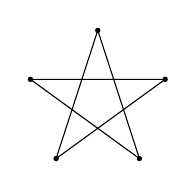
\begin{tikzpicture}[scale=0.75]
\foreach \k in {0,...,4}{\coordinate (v\k) at ({90+72*\k}:1.2);}
\draw (v0)--(v2)--(v4)--(v1)--(v3)--cycle;
\foreach \k in {0,...,4}{\fill (v\k) circle (1.3pt);}
\end{tikzpicture}
\end{center}
The group of symmetries of the regular pentagram shown above is isomorphic to the
\begin{enumerate}[label=(\Alph*)]
\item symmetric group $S_5$
\item alternating group $A_5$
\item cyclic group of order $5$
\item cyclic group of order $10$
\item dihedral group of order $10$
\end{enumerate}
\textbf{名词解释。}regular pentagram：正五角星；symmetry：保持图形的对称变换；group of symmetries：以变换复合为运算的对称群；isomorphic：同构；order of a group：群中元素个数；dihedral group：二面体群。这里的 symmetric group $S_5$ 是“对称群／置换群”的专有名词，不是说任何图形的对称群都等于 $S_5$。

\textbf{先回顾群的定义。}集合 $G$ 配备一个运算，若运算封闭、满足结合律、存在单位元且每个元素都有逆元，则称为群。图形对称变换的复合仍保持图形，什么都不做是单位元，每个旋转或反射都可以逆转，所以这些变换构成群。群同构是一个双射 $\varphi:G\to H$，还要求 $\varphi(ab)=\varphi(a)\varphi(b)$；不仅数目相同，运算结构也要相同。

\textbf{先数旋转。}绕中心旋转 $0^\circ,72^\circ,144^\circ,216^\circ,288^\circ$ 都保持五角星，共 5 个。令 $r$ 表示旋转 $72^\circ$，这 5 个变换是 $e,r,r^2,r^3,r^4$，且 $r^5=e$。

\textbf{再数反射。}有 5 条反射对称轴，每条经过一个外顶点和中心。令 $s$ 为其中一次反射，则其余反射可写为 $rs,r^2s,r^3s,r^4s$。所有平面对称共 10 个：5 个旋转和 5 个反射。这里计入整个图形的平面等距变换，不是对五个顶点任意重新编号。

\textbf{为什么是二面体群？}它与正五边形的对称群相同，满足
\[
r^5=e,\qquad s^2=e,\qquad srs=r^{-1}.
\]
最后一个关系表示“反射会把旋转方向反过来”。这是阶为 10 的二面体群，选 E。不同教材可能记作 $D_5$ 或 $D_{10}$，应以“阶为 10”识别，避免记号混淆。

\textbf{逐项排除。}A：$|S_5|=5!=120$，它允许任意置换，太多。B：$|A_5|=5!/2=60$，它只含偶置换，数量仍不对。C：阶 5 的循环群只描述旋转，漏了反射。D：阶 10 的循环群必须有一个阶 10 的生成元，但此处非恒等旋转的阶都是 5，反射的阶都是 2，没有阶 10 的元素；而且此群不交换，循环群必交换。因此不能只凭“有 10 个元素”选择 D。

\textbf{举一反三。}正 $n$ 边形的平面对称群有 $2n$ 个元素，包含 $n$ 个旋转与 $n$ 个反射；只允许旋转时得到阶 $n$ 的循环群。注意区分群的阶 $|G|$ 与元素的阶 $\operatorname{ord}(g)$（最小正整数 $k$ 使 $g^k=e$）。

\subsection{65. 连续满射与连续双射：B}
\label{p2:q65}
\textbf{原题（Original problem）}

Which of the following statements are true about the open interval $(0,1)$ and the closed interval $[0,1]$?
\begin{enumerate}[label=\Roman*.]
\item There is a continuous function from $(0,1)$ onto $[0,1]$.
\item There is a continuous function from $[0,1]$ onto $(0,1)$.
\item There is a continuous one-to-one function from $(0,1)$ onto $[0,1]$.
\end{enumerate}
(A) None \quad (B) I only \quad (C) II only \quad (D) I and III only \quad (E) I, II, and III.

\textbf{审题重点。}from 指定义域，onto 指满射，要求\emph{值域恰好等于}后面的集合；one-to-one 指单射，即不同输入有不同输出。I 只要求连续满射，允许重复取值；III 同时要求连续、单射、满射，明显比 I 强。``There is'' 是存在至少一个函数，不是每个函数都满足。

\textbf{I 正确：直接构造。}令
\[
f:(0,1)\to[0,1],\qquad f(x)=\sin^2(2\pi x).
\]
它连续且值总在 $[0,1]$。在定义域内的点上，$f(\frac14)=1$、$f(\frac12)=0$。由介值定理，在 $[\frac14,\frac12]\subset(0,1)$ 上能取到 0 与 1 之间每个值，所以满射到 $[0,1]$。目标集合包含端点，并不要求定义域也包含端点；输出为 0 或 1 的输入可以是内部点。

\textbf{II 错误：连续函数在闭有界区间上达到最值。}若连续 $g:[0,1]\to(0,1)$ 为满射，则其值域应为 $(0,1)$。但极值定理保证存在 $a,b\in[0,1]$，使 $m=g(a)$ 是最小值、$M=g(b)$ 是最大值。由于所有函数值都在 $(0,1)$，有 $0<m\le M<1$。例如 $m/2\in(0,1)$ 不可能被取到，与满射矛盾。也可说紧集 $[0,1]$ 的连续像必须紧，而 $(0,1)$ 不紧。

\textbf{III 错误：单射造成障碍。}反设存在连续单射满射 $h:(0,1)\to[0,1]$。满射要求存在 $a\in(0,1)$ 使 $h(a)=0$。选 $u<a<v$，都在 $(0,1)$ 中。由于单射且函数值非负，$h(u)>0$、$h(v)>0$。取 $c=\frac12\min\{h(u),h(v)\}>0$。介值定理分别作用于 $[u,a]$ 和 $[a,v]$，得到 $u<\xi<a<\eta<v$ 且 $h(\xi)=h(\eta)=c$，与单射矛盾。因此不存在这样的 $h$。

相关结论是：实区间上的连续单射必严格单调；而开区间上的严格单调函数不可能在内部取得全局最小值 0 和最大值 1。只知道两个集合等势（存在集合意义的双射），不能推断存在连续双射。最终只有 I 正确，选 B。

\subsection{66. 只有两个右理想的含幺环：B}
\label{p2:q66}
\textbf{原题（Original problem）}

Let $R$ be a ring with a multiplicative identity. If $U$ is an additive subgroup of $R$ such that $ur\in U$ for all $u\in U$ and for all $r\in R$, then $U$ is said to be a right ideal of $R$. If $R$ has exactly two right ideals, which of the following must be true?
\begin{enumerate}[label=\Roman*.]
\item $R$ is commutative.
\item $R$ is a division ring (that is, all elements except the additive identity have multiplicative inverses).
\item $R$ is infinite.
\end{enumerate}
(A) I only \quad (B) II only \quad (C) III only \quad (D) I and II only \quad (E) I, II, and III.

\textbf{先回顾定义。}环的加法构成交换群，乘法满足结合律，且乘法对加法满足左右分配律。含幺环（ring with a multiplicative identity）另有元素 $1$ 满足 $1r=r1=r$。加法单位元是 $0$，不要与乘法单位元 $1$ 混淆。

加法子群 $U$ 满足 $0\in U$ 且 $u-v\in U$（$u,v\in U$）。右理想在此基础上还要求 $ur\in U$（$u\in U,r\in R$），即理想元素放左边，右乘任意环元素后仍在理想中。左理想要求 $ru\in U$；双侧理想两个方向都要求。除环（division ring）是 $1\ne0$ 且每个非零元素均有双侧乘法逆元的环，\emph{不要求}乘法交换；再要求乘法交换才是域（field）。

\textbf{第一步：恰好是哪两个右理想？}$\{0\}$ 和 $R$ 永远是右理想。若 $R$ 为零环，它们相同，只有一个右理想；本题恰有两个，故 $1\ne0$，且只有 $\{0\}$、$R$ 两个右理想。

\textbf{第二步：从任意非零元素构造右理想。}任取 $a\ne0$，考虑
\[
aR=\{ar:r\in R\}.
\]
它是右理想：$0=a0\in aR$；$ar_1-ar_2=a(r_1-r_2)\in aR$；$(ar)t=a(rt)\in aR$。又因为 $a=a1\in aR$ 且 $a\ne0$，所以它不是零理想，只能有 $aR=R$。因此 $1\in aR$，存在 $b\in R$ 使
\begin{equation}
ab=1.
\label{p2:right-inverse}
\end{equation}
这只先证明 $b$ 是 $a$ 的\emph{右逆}，不能未经证明就改写为 $ba=1$。

\textbf{第三步：把右逆变成双侧逆。}由 $ab=1$ 知 $b\ne0$，对 $b$ 重复第二步，得到某个 $c\in R$ 使 $bc=1$。由结合律，
\[
a=a(bc)=(ab)c=c.
\]
于是 $ba=bc=1$。结合 $ab=1$，得到 $b$ 是 $a$ 的双侧逆。由于 $a\ne0$ 任意，所有非零元素都可逆，II 正确。

\textbf{I 不一定成立。}实四元数环 $\mathbb H=\{a+bi+cj+dk:a,b,c,d\in\mathbb R\}$ 是非交换除环，其乘法满足 $i^2=j^2=k^2=-1$、$ij=k$、$ji=-k$。每个非零四元数 $q=a+bi+cj+dk$ 都有逆
\[
q^{-1}=\frac{a-bi-cj-dk}{a^2+b^2+c^2+d^2}.
\]
除环的非零右理想若含 $q\ne0$，由右吸收性含 $qq^{-1}=1$，继而含 $1r=r$（任意 $r\in R$），所以必为整个环。因此四元数环恰有两个右理想，却不交换，否定 I。GRE 中需要认识这个标准反例，不必在本题展开构造四元数乘法。

\textbf{III 不一定成立。}有限域 $\mathbb F_2=\mathbb Z/2\mathbb Z=\{0,1\}$ 有乘法单位元，唯一非零元素 1 可逆，故恰有两个右理想，却是有限集合。因此 III 错。只有 II 必然成立，选 B。

\textbf{举一反三。}含幺非零环中，只要某个右理想包含 1，它就等于整个环。交换含幺非零环只有两个理想，当且仅当它是域；不预设交换时，只有两个\emph{右}理想推出除环。不要把条件擅自弱化成“只有两个\emph{双侧}理想”：矩阵环 $M_n(\mathbb R)$（$n\ge2$）只有零理想与全环两个双侧理想，但包含非零不可逆矩阵，不是除环。左右条件在非交换环中确实重要。

\subsection{本套复习清单}
\begin{itemize}
\item 18、26：把 onto、relative、absolute 等词先译准，再套定理；矩阵空间维数与矩阵秩必须分开。
\item 36、58：区分两两无关与整体无关；相似矩阵保持迹，优先写出 $B=S^{-1}AS$。
\item 47：从功的线积分出发；恒力用力与位移的点积，不能用力的大小乘路程。
\item 48：逐步检查中值定理条件、不等号方向和固定正下界，不靠图形感觉判断论证。
\item 60、66：先记群、群的阶、循环群、二面体群，以及右理想、除环、域的定义；反例分别记正五边形对称群、四元数环和有限域。
\item 65：把 from、onto、one-to-one 分开读。连续满射可以重复取值；紧集的连续像是紧集。
\end{itemize}
\clearpage
\section{GRE Mathematics 错题与不确定题：Practice 3}
本节收录 7、48、55、56、59、62，共 6 题。其中 48、55、59 按自述为答对但不确定；7 重点为词义，56 为已经自行理解后再巩固，62 为广义拓扑知识缺口。这里的收录数量不代表实际错题数，不额外推断整套成绩。原题及选项核对所附试卷 Form GR9367；答案依次为 D、D、E、B、A、B。

\subsection{7. Octants：三维空间的八个卦限：D}
\label{p3:q7}
\textbf{原题（Original problem）}

In how many of the eight standard octants of $xyz$-space does the graph of $z=e^{x+y}$ appear?

(A) One \quad (B) Two \quad (C) Three \quad (D) Four \quad (E) Eight.

\textbf{名词解释。}octant：卦限，也称八分空间（one of the eight regions determined by the signs of $x,y,z$）；octants 是复数。二维中两个坐标轴把平面分成四个 quadrant（象限）；三维中三个坐标平面 $x=0,y=0,z=0$ 把空间分成八个 octant。graph：函数图像，本题是空间曲面，不是平面曲线。坐标平面是这些区域的边界，不影响这里的计数。

\textbf{解答。}八个卦限分别对应 $(x,y,z)$ 的正负号组合，共 $2^3=8$ 种。因为指数函数恒正，
\[
z=e^{x+y}>0,
\]
所以图像不可能进入任何 $z<0$ 的卦限。但 $x,y$ 可任取正数或负数，故下列四种组合都能出现：
\[
(+,+,+),\quad (+,-,+),\quad (-,+,+),\quad (-,-,+).
\]
例如分别取 $(x,y)=(1,1),(1,-1),(-1,1),(-1,-1)$，都能得到对应的 $z>0$。因此恰好出现于 4 个卦限，选 D；A--C 少算了可能的 $x,y$ 符号，E 则错误地计入 $z<0$ 的区域。

\textbf{可迁移的方法。}遇到 quadrant/octant，先逐个检查各坐标能否为正、为负，不需要先画精确图像。$z>0$ 只限制高度，不能据此把 $x,y$ 也限制为正。

\subsection{48. 有限循环群直积何时仍循环：D（答对但不确定）}
\label{p3:q48}
\textbf{原题（Original problem）}

Let $G_n$ denote the cyclic group of order $n$. Which of the following direct products is NOT cyclic?
\begin{enumerate}[label=(\Alph*)]
\item $G_{17}\times G_{11}$
\item $G_{17}\times G_{11}\times G_5$
\item $G_{17}\times G_{33}$
\item $G_{22}\times G_{33}$
\item $G_{49}\times G_{121}$
\end{enumerate}
\textbf{名词解释。}cyclic group：循环群，存在某个元素，其整数次幂生成全群；order of a group：群的阶（元素个数）；order of an element：元素的阶，即最小正整数 $k$ 使 $g^k=e$；direct product：直积；coprime / relatively prime：互质；gcd：最大公因数；lcm：最小公倍数。

\textbf{从直积定义出发。}$G\times H$ 的元素是有序对，按分量运算：$(g,h)(g',h')=(gg',hh')$，所以 $(g,h)^k=(g^k,h^k)$。若 $g,h$ 的阶分别为 $r,s$，则这个有序对回到单位元，当且仅当 $r\mid k$ 且 $s\mid k$。因此
\begin{equation}
\operatorname{ord}(g,h)=\operatorname{lcm}(r,s).
\label{p3:product-element-order}
\end{equation}

\textbf{循环性的判据与证明。}有限循环群 $G_m,G_n$ 的直积共有 $mn$ 个元素。取两个因子的生成元 $g,h$，则 $(g,h)$ 的阶为 $\operatorname{lcm}(m,n)=mn/\gcd(m,n)$。若 $\gcd(m,n)=1$，它的阶就是 $mn$，故可生成整个直积。反过来，任意元素的两个分量的阶分别整除 $m,n$，故其阶至多为 $\operatorname{lcm}(m,n)$。若 $\gcd(m,n)>1$，这个数小于 $mn$，没有任何元素能生成整个直积。因此
\begin{equation}
G_m\times G_n\text{ 是循环群}\quad\Longleftrightarrow\quad\gcd(m,n)=1.
\label{p3:cyclic-product}
\end{equation}

\textbf{逐项核对。}A：17 与 11 互质，循环。B：17、11、5 两两互质，取三个生成元构成的元素，其阶为 $17\cdot11\cdot5$，循环。C：$33=3\cdot11$，与 17 互质，循环。D：$22=2\cdot11$、$33=3\cdot11$，最大公因数为 11，不循环。E：$49=7^2$、$121=11^2$ 互质，循环。故选 D，你关于 22 和 33 不互质的判断是正确的。

\textbf{本题的数量检查。}$|G_{22}\times G_{33}|=726$，但任意元素的阶至多为 $\operatorname{lcm}(22,33)=66$，所以不可能有阶为 726 的生成元。最小例子是 $G_2\times G_2$：虽然有 4 个元素，每个非单位元素的阶却都是 2，因此它不同构于 $G_4$。多个有限循环群的直积循环，当且仅当各因子的阶两两互质；仅有所有阶数的总 gcd 为 1 不够。

\subsection{55. 整数加法群的子群与整除：E（答对但不确定）}
\label{p3:q55}
\textbf{原题（Original problem）}

Let $p$ and $q$ be distinct primes. There is a proper subgroup $J$ of the additive group of integers which contains exactly three elements of the set $\{p,p+q,pq,p^q,q^p\}$. Which three elements are in $J$?
\begin{enumerate}[label=(\Alph*)]
\item $pq,p^q,q^p$
\item $p+q,pq,p^q$
\item $p,p+q,pq$
\item $p,p^q,q^p$
\item $p,pq,p^q$
\end{enumerate}
\textbf{名词解释。}distinct primes：不同的素数，所以 $\gcd(p,q)=1$；additive group of integers：整数在加法运算下组成的群 $(\mathbb Z,+)$；proper subgroup：真子群，即子群但不等于整个群；exactly three：恰好三个，多一个或少一个都不行。注意 $p^q$ 是 $p$ 的 $q$ 次幂，不是乘积 $pq$。

\textbf{先回顾子群。}加法子群 $J\subseteq\mathbb Z$ 必须包含 0，且 $a,b\in J$ 时 $a-b\in J$；因此可以做任意整数倍和整数线性组合。整数加法群的每个子群都形如
\[
n\mathbb Z=\{nk:k\in\mathbb Z\},\qquad n\ge0.
\]
若子群不是 $\{0\}$，取其中最小的正整数 $n$；对任意 $a\in J$ 作带余除法 $a=kn+r$、$0\le r<n$，则 $r=a-kn\in J$。最小性迫使 $r=0$，故每个元素均为 $n$ 的倍数；反向由加法封闭得到所有 $n$ 的倍数均在 $J$。这就证明上述结论。本题子群含有三个正整数，因此非零，又是真子群，所以 $J=n\mathbb Z$ 且 $n\ge2$。

\textbf{先构造 E。}取 $J=p\mathbb Z$。那么 $p,pq,p^q$ 都是 $p$ 的倍数，因此在 $J$ 中；$p+q$ 除以 $p$ 的余数与 $q$ 相同，不为零；$q^p$ 也不被 $p$ 整除。因此恰好包含 $p,pq,p^q$，E 可行。

\textbf{为什么别的三元组合不行？}若一个整数加法子群同时含 $a,b$，则也含 $\gcd(a,b)$，因为贝祖等式给出 $ua+vb=\gcd(a,b)$。若这个 gcd 为 1，就含 1，进而含所有整数，与真子群矛盾。A 中 $p^q,q^p$ 互质；B 中 $p+q,pq$ 互质；C 中 $p,p+q$ 互质；D 中 $p,q^p$ 互质。因此 A--D 都会强迫 $J=\mathbb Z$，均不可能，只有 E 正确。

\textbf{一个数值例子。}令 $p=2,q=3$，原集合成为 $\{2,5,6,8,9\}$。真子群 $2\mathbb Z$ 恰含其中的 $2,6,8$。若同时含 8 和 9，则也含 $9-8=1$，不再是真子群。

\textbf{与上一题的区别。}整数加法群中由整数 $a,b$ 生成的子群是 $\gcd(a,b)\mathbb Z$；它们的倍数集合之交是 $a\mathbb Z\cap b\mathbb Z=\operatorname{lcm}(a,b)\mathbb Z$（$a,b>0$）。生成子群用 gcd，交集用 lcm，直积元素的阶用 lcm，不能仅凭题目里出现两个整数就选同一个公式。

\subsection{56. 导集、闭包与反例：B}
\label{p3:q56}
\textbf{原题（Original problem）}

For a subset $S$ of a topological space $X$, let $\operatorname{cl}(S)$ denote the closure of $S$ in $X$, and let $S'=\{x:x\in\operatorname{cl}(S-\{x\})\}$ denote the derived set of $S$. If $A$ and $B$ are subsets of $X$, which of the following statements are true?
\begin{enumerate}[label=\Roman*.]
\item $(A\cup B)'=A'\cup B'$.
\item $(A\cap B)'=A'\cap B'$.
\item If $A'$ is empty, then $A$ is closed in $X$.
\item If $A$ is open in $X$, then $A'$ is not empty.
\end{enumerate}
(A) I and II only \quad (B) I and III only \quad (C) II and IV only \quad (D) I, II, and III only \quad (E) I, II, III, and IV.

\textbf{名词解释。}closure：闭包；derived set：导集，即全部聚点组成的集合，这里的撇号不是求导；accumulation point / limit point：聚点；neighborhood：邻域；empty：空的。聚点不要求属于原集合。

\textbf{先用邻域理解定义。}$x\in\operatorname{cl}(S)$，指每个包含 $x$ 的开邻域都与 $S$ 相交；$x\in S'$，指每个包含 $x$ 的开邻域都与 $S\setminus\{x\}$ 相交，不能仅靠 $x$ 自己证明它是聚点。与此相对，$x\in S$ 若有一个邻域只在 $x$ 处碰到 $S$，则称为孤立点。例如 $S=\{0\}\cup\{1/n:n\ge1\}$ 在通常实数拓扑中有 $S'=\{0\}$，而每个 $1/n$ 都是孤立点。

\textbf{I 正确。}若 $x\in A'$，则每个邻域都碰到 $A\setminus\{x\}$，自然也碰到 $(A\cup B)\setminus\{x\}$，故 $A'\cup B'\subseteq(A\cup B)'$。反向用逆否：若 $x\notin A'\cup B'$，则存在开邻域 $U,V$ 分别不碰 $A\setminus\{x\}$、$B\setminus\{x\}$。开邻域 $U\cap V$ 就不碰 $(A\cup B)\setminus\{x\}$，所以 $x\notin(A\cup B)'$。两边包含得到等号。

\textbf{II 错误，你的反例成立。}取 $X=\mathbb R$ 配通常拓扑，$A=\mathbb Q$、$B=\mathbb R\setminus\mathbb Q$。两者不交，所以 $(A\cap B)'=\varnothing'=\varnothing$。但任意实数的每个开区间邻域都包含\emph{其他}有理数及\emph{其他}无理数，故 $A'=B'=\mathbb R$，从而 $A'\cap B'=\mathbb R$。因此左边空、右边全空间，不相等。一般只有 $(A\cap B)'\subseteq A'\cap B'$：分别能在邻域内找到 $A$ 的点和 $B$ 的点，不表示能找到同时属于二者的点。

\textbf{III 正确。}任何拓扑空间中都有
\begin{equation}
\operatorname{cl}(A)=A\cup A'.
\label{p3:closure-derived}
\end{equation}
证明：$A\subseteq\operatorname{cl}(A)$，$A'\subseteq\operatorname{cl}(A)$。反过来，若 $x\in\operatorname{cl}(A)$ 且 $x\notin A$，则 $A\setminus\{x\}=A$，故 $x\in\operatorname{cl}(A\setminus\{x\})$，即 $x\in A'$。因此 $A'=\varnothing$ 蕴含 $\operatorname{cl}(A)=A$，所以 $A$ 闭。不要反过来理解成“闭集的导集一定为空”；例如 $[0,1]'=[0,1]$。

\textbf{IV 错误，你给的空集反例足够。}取 $A=\varnothing$；空集在任何拓扑空间中都既开又闭，而且 $A'=\varnothing$。所以“开就必有聚点”不成立。甚至补充非空也未必对：在离散拓扑中，单点集开，但没有聚点。最终只有 I、III 正确，选 B。

\textbf{记忆。}有限并的导集可分配；交集只有包含关系。$A$ 闭等价于 $A'\subseteq A$，并非 $A'=\varnothing$。注意这些结论在本题给定的导集定义下成立，不需要先假设 $X$ 是通常的欧氏空间。

\subsection{59. 由两个有限子群生成的群的阶：A（答对但不确定）}
\label{p3:q59}
\textbf{原题（Original problem）}

Two subgroups $H$ and $K$ of a group $G$ have orders 12 and 30, respectively. Which of the following could NOT be the order of the subgroup of $G$ generated by $H$ and $K$?

(A) 30 \quad (B) 60 \quad (C) 120 \quad (D) 360 \quad (E) Countable infinity.

\textbf{名词解释。}subgroup generated by $H$ and $K$：由 $H,K$ 生成的子群，记作 $L=\langle H\cup K\rangle$，即包含二者的最小子群，其元素是来自 $H,K$ 的有限乘积；could NOT：不可能；countable infinity：可数无限，即元素可按自然数编号。这里不是问 $H\cap K$，也不是问某一个直积元素的阶。

\textbf{先用拉格朗日定理。}因为 $H,K$ 都是 $L$ 的子群，若 $L$ 有限，则
\[
12\mid|L|,\qquad30\mid|L|,
\qquad\text{故}\quad\operatorname{lcm}(12,30)=60\mid|L|.
\]
30 不是 12 的倍数，因此不可能；选 A。你的 lcm 思路抓住了必要条件，但结论应是“有限时阶数必须是 60 的倍数”，不是“一定恰好等于 60”。

\textbf{为什么其余选项确实可能？}60 可以取循环群 $C_{60}=\langle g\rangle$，其中 $H=\langle g^5\rangle$ 的阶为 12，$K=\langle g^2\rangle$ 的阶为 30；由于 $g=g^5(g^2)^{-2}$，二者生成整个 $C_{60}$。

120、360 可以用二面体群给出具体构造。设 $D_N=\langle r,s:r^N=s^2=e,\ srs=r^{-1}\rangle$，它是正 $N$ 边形的对称群，\emph{阶为 $2N$}。当 $N=60$ 或 $180$ 时，令
\[
H=\langle r^{N/6},s\rangle,\qquad K=\langle r^{N/15},rs\rangle.
\]
$H$ 有 6 个旋转和 6 个反射，阶为 12；$K$ 有 15 个旋转和 15 个反射，阶为 30。二者合起来含有 $s$、$rs$，故含 $(rs)s=r$，于是生成整个 $D_N$，给出阶为 120 和 360 的例子。这些构造用于核实选项；考场上先用整除关系排除 A 即可。

\textbf{可数无限也可能。}标准例子是自由积 $C_{12}*C_{30}$，其中自然包含阶为 12 和 30 的两个循环子群。直观上，其元素可以写成来自两个因子的非单位元素交替排列的有限单词；除了各因子内部的关系，不另加交换等关系。若 $a,b$ 分别是两个因子的生成元，则 $(ab)^k$（$k=1,2,\ldots$）是互不相同的约化单词，因此群无限；而有限字母表上的有限单词总共可数，所以它是可数无限群。这里认识这种可能性即可，不必为本题系统学习自由积。

\textbf{与直积题区分。}第 \ref{p3:q48} 题中，$(g,h)$ 是一个\emph{直积元素}，它的阶精确等于两个分量阶的 lcm。本题的 $L$ 允许 $H,K$ 的元素交替相乘，没有预设这些元素彼此交换，因此不能直接套直积公式。若已知 $G$ 是阿贝尔群，则 $L=HK$ 且 $|L|=|H||K|/|H\cap K|$；一般群中 $HK$ 未必是子群，不能把这个集合的大小直接当作 $|L|$。

\subsection{62. 下限拓扑、Hausdorff、紧性和连通性：B}
\label{p3:q62}
\textbf{原题（Original problem）}

Let $R$ be the set of real numbers with the topology generated by the basis $\{[a,b):a<b,\text{ where }a,b\in R\}$. If $X$ is the subset $[0,1]$ of $R$, which of the following must be true?
\begin{enumerate}[label=\Roman*.]
\item $X$ is compact.
\item $X$ is Hausdorff.
\item $X$ is connected.
\end{enumerate}
(A) I only \quad (B) II only \quad (C) III only \quad (D) I and II \quad (E) II and III.

\textbf{先说明什么是拓扑。}在集合 $Y$ 上指定一族子集 $\tau$ 作为开集，要求：$\varnothing,Y\in\tau$；任意多个开集之并仍开；有限多个开集之交仍开。集合连同这种开集规则称为拓扑空间 $(Y,\tau)$。所以开集不是由集合本身的形状决定的；同一个 $\mathbb R$ 配上不同拓扑，可以有不同的开集、连续性、紧性和连通性。

\textbf{什么是基？}一族基本开集构成基，意思是所有开集都由基本开集任意取并得到。本题以左闭右开的 $[a,b)$ 为基本开集，称下限拓扑（lower limit topology），实数集合配此拓扑称 Sorgenfrey line。虽然 $[a,b)$ 在通常实数拓扑中不是开集，但在本题中它按定义就是开集；不能把书写中的方括号直接等同于拓扑意义上的闭集。

\textbf{子空间拓扑。}题目中的 $X=[0,1]$ 继承此拓扑：$U\subseteq X$ 在 $X$ 中开，当且仅当可写成 $U=X\cap O$，其中 $O$ 是原空间中的开集。例如 $\{1\}=X\cap[1,2)$，因此 $\{1\}$ 在 $X$ 中开；这与通常的闭区间拓扑不同。

\textbf{II 正确：Hausdorff 的定义与验证。}Hausdorff（豪斯多夫，或 $T_2$）要求任意两个不同的点都能被不相交的开邻域分开：若 $x\ne y$，则存在开集 $U,V$，使
\[
x\in U,\quad y\in V,\quad U\cap V=\varnothing.
\]
任取 $x<y$，可直接取 $U=[x,y)$、$V=[y,y+1)$；它们都是原空间的开集，不相交且分别包含 $x,y$。与 $X$ 取交后仍是所需的子空间开邻域，所以 $X$ 是 Hausdorff。通常的度量空间都 Hausdorff，但满足 Hausdorff 不意味着一定在使用通常的欧氏拓扑。

\textbf{I 错误：用开覆盖证明不紧。}compact（紧）的定义是每个开覆盖都有有限子覆盖。考虑 $X$ 的开集族
\[
\mathcal U=\{[0,1-1/n):n=2,3,\ldots\}\cup\{\{1\}\}.
\]
每个 $x<1$ 都小于某个 $1-1/n$，所以这些半开区间覆盖 $[0,1)$；单点集 $\{1\}$ 覆盖最后的端点，因此是开覆盖。但有限选取时，令其中最大的下标为 $N$，所选区间的并至多为 $[0,1-1/N)$；再加上 $\{1\}$ 仍漏掉 $[1-1/N,1)$。因此没有有限子覆盖，$X$ 不紧。若一个半开区间都没选，更不可能覆盖。欧氏空间的“闭且有界当且仅当紧”只适用于通常拓扑，不能不检查拓扑就套到这里。

\textbf{III 错误：构造分离。}connected（连通）指不能写成两个不交、非空的相对开集之并。这里
\[
X=[0,1/2)\ \cup\ [1/2,1].
\]
第一部分是基本开集与 $X$ 的交；第二部分为 $X\cap[1/2,2)$，也在 $X$ 中开。二者不交且非空，合起来为 $X$，所以 $X$ 不连通。最终只有 II 正确，选 B。

\textbf{可迁移的检查顺序。}先明确“什么集合算开集”，再按定义检查性质：Hausdorff 要把两个点用开邻域分开；不紧可找没有有限子覆盖的开覆盖；不连通可找两个不交非空开集覆盖全空间。不要因为集合写成 $[0,1]$ 就直接认为它紧且连通。

\subsection{本套复习定位}
\begin{itemize}
\item 7：补词义 octant；用坐标正负号计数。
\item 48：循环群直积的阶是因子阶之积，直积中单个元素的阶是分量阶的 lcm；要有生成元，两者必须能相等。
\item 55：整数加法子群全为 $n\mathbb Z$；真子群不能含 1；贝祖等式可快速排除互质元素同时出现的选项。
\item 56：你的有理／无理数反例和空集反例都成立；再把有限并公式与闭包公式的证明掌握。
\item 59：lcm 是有限生成子群阶数的整除约束，不是一般情形的精确阶数；保留可数无限的可能性。
\item 62：系统补齐拓扑、基、子空间拓扑、Hausdorff、开覆盖紧性、连通的定义，再做非常规拓扑题。
\end{itemize}

\clearpage
\section{GRE Mathematics 错题与不确定题：Practice 4}
本套 Form GR8767 共 66 题。按每题题号旁的蓝笔选项再次逐一核对卷末答案表，答对 64 题、错 2 题：17 题选 E，正确答案 C；53 题选 C，正确答案 B。其余 64 题均与答案表一致。本节另收录答对但需要巩固的 55、58、60、64，共整理 6 题；收录数不等于错题数。

\subsection{17. 自定义运算的逆元：分母为零不能漏检：C}
\label{p4:q17}
\textbf{原题（Original problem）}

Let $*$ be the binary operation on the rational numbers given by $a*b=a+b+2ab$. Which of the following are true?
\begin{enumerate}[label=\Roman*.]
\item $*$ is commutative.
\item There is a rational number that is a $*$-identity.
\item Every rational number has a $*$-inverse.
\end{enumerate}
(A) I only \quad (B) II only \quad (C) I and II only \quad (D) I and III only \quad (E) I, II, and III.

\textbf{名词解释。}binary operation：二元运算，给两个输入得到一个输出；commutative：交换的；$*$-identity：关于本题运算 $*$ 的单位元；$*$-inverse：关于 $*$ 的逆元。单位元与逆元必须按新运算求，不能自动当成普通乘法的 1 和倒数。

\textbf{错因记录。}实际选 E。已经算出了逆元的候选公式，但没有检查分母为零的 $a=-\frac12$。这是定义域中特殊值遗漏，而非没有掌握逆元的定义。

\textbf{I 正确。}普通有理数加法、乘法交换，所以 $a*b=a+b+2ab=b+a+2ba=b*a$。

\textbf{II 正确。}设单位元为 $e$，要求对所有 $a\in\mathbb Q$，$a*e=a$，即 $e(1+2a)=0$。取 $a=0$ 得 $e=0$；再验证 $a*0=0*a=a$，故单位元是 0。

\textbf{III 错误。}元素 $a$ 的逆元 $b$ 必须满足 $a*b=0$，即
\[
a+b+2ab=0\quad\Longleftrightarrow\quad(1+2a)b=-a.
\]
只有 $1+2a\ne0$ 时，才能除以它并写成
\[
b=-\frac{a}{1+2a}.
\]
此时若 $a$ 有理，$b$ 也有理。但当 $a=-\frac12$ 时，对任意 $b\in\mathbb Q$，
\[
-\frac12*b=-\frac12+b-b=-\frac12\ne0,
\]
因此 $-\frac12$ 没有逆元。只有 I、II 正确，选 C。

\textbf{检查动作。}出现含变量的分母时，把“分母为零”单独列成一类，并确认该值是否在题目定义域中；不能只得到一个形式上的公式就宣布所有元素都有逆元。对本题还可观察 $1+2(a*b)=(1+2a)(1+2b)$：$a=-\frac12$ 对应右端的零因子，恰好解释其不可逆性。

\subsection{53. 多项式空间与零自由度：B}
\label{p4:q53}
\textbf{原题（Original problem）}

Let $V$ be the vector space, under the usual operations, of real polynomials that are of degree at most 3. Let $W$ be the subspace of all polynomials $p(x)$ in $V$ such that $p(0)=p(1)=p(-1)=0$. Then $\dim V+\dim W$ is

(A) 4 \quad (B) 5 \quad (C) 6 \quad (D) 7 \quad (E) 8.

\textbf{名词解释。}degree at most 3：次数至多为 3，包含低次多项式及零多项式；usual operations：通常的多项式加法与实数数乘；dimension：维数，即自由参数个数或一组基的元素个数；unique：唯一。

\textbf{错因记录。}实际选 C，把 $\dim W$ 算成了 2。原思路把“唯一解”误当作一维；但唯一解没有任何可自由选择的参数，对应零自由度。在本题这种齐次线性条件下，若只有零多项式一个解，就得到零空间 $\{0\}$，其维数为 0，而不是 1。

\textbf{直接用因式分解。}$V$ 的基为 $1,x,x^2,x^3$，所以 $\dim V=4$。$p$ 在三个不同点 $0,1,-1$ 处为零，故 $x(x-1)(x+1)$ 整除 $p$。由于次数至多为 3，必有
\[
p(x)=c\,x(x-1)(x+1)=c(x^3-x),\qquad c\in\mathbb R.
\]
因此 $W=\operatorname{span}\{x^3-x\}$，只有一个自由参数，$\dim W=1$，故所求为 $4+1=\boxed5$，选 B。

\textbf{也可直接求系数。}写 $p(x)=a_0+a_1x+a_2x^2+a_3x^3$，则
\[
a_0=0,\qquad a_1+a_2+a_3=0,\qquad -a_1+a_2-a_3=0.
\]
后两式相加得 $a_2=0$，再得 $a_1=-a_3$，所以只剩 $a_3$ 一个自由参数。

\textbf{纠正维数的直觉。}一个含任意实参数的直线有无穷多个点，但维数为 1；只有零向量的子空间只含一个点，维数为 0。条件数与维数的关系是“维数减去\emph{独立线性约束的个数}”，不能每看到一个条件就机械减 1，重复条件不会继续降维。若次数至多为 $n$ 的多项式被要求在 $k$ 个不同实点为零，则 $k\le n+1$ 时这 $k$ 个取值约束独立，满足条件的空间维数为 $n+1-k$；若 $k\ge n+1$，只有零多项式，维数为 0。

\subsection{55. Hessian 判别：先看行列式，再看符号：C（答对后巩固）}
\label{p4:q55}
\textbf{原题（Original problem）}

Let $f(x,y)=x^3+y^3+3xy$ for all real $x$ and $y$. Then there exist distinct points $P$ and $Q$ such that $f$ has a
\begin{enumerate}[label=(\Alph*)]
\item local maximum at $P$ and at $Q$
\item saddle point at $P$ and at $Q$
\item local maximum at $P$ and a saddle point at $Q$
\item local minimum at $P$ and a saddle point at $Q$
\item local minimum at $P$ and at $Q$
\end{enumerate}
\textbf{名词解释。}Hessian matrix：海森矩阵，即由二阶偏导数组成的矩阵；critical/stationary point：驻点；local maximum/minimum：局部极大／极小值；saddle point：鞍点，附近既有更大值也有更小值。

\textbf{作答记录。}开始不确定，后来独立用二阶偏导判别做对，选 C。记忆中“行列式小于零是鞍点”是正确的；“行列式大于零”还需检查另一个符号，才能区分极大和极小。

\textbf{第一步：找出全部驻点。}
\[
f_x=3x^2+3y=0,\qquad f_y=3y^2+3x=0.
\]
由 $y=-x^2$，代入第二式得 $x^4+x=0$，即 $x(x^3+1)=0$。实数解只有 $x=0,-1$，相应驻点为 $(0,0)$ 和 $(-1,-1)$。

\textbf{第二步：计算 Hessian。}
\[
H_f(x,y)=\begin{pmatrix}6x&3\\3&6y\end{pmatrix},
\qquad D=f_{xx}f_{yy}-f_{xy}^2=36xy-9.
\]
在 $(0,0)$，$D=-9<0$，故为鞍点。在 $(-1,-1)$，$D=27>0$ 且 $f_{xx}=-6<0$，故为严格局部极大值点。于是取 $P=(-1,-1)$、$Q=(0,0)$，选择 C；没有局部极小值，也没有两个局部极大值或两个鞍点，故其余选项均错。

\textbf{完整判别表。}对二元 $C^2$ 函数的驻点：
\[
\begin{array}{c|c}
\text{条件}&\text{结论}\\\hline
D<0&\text{鞍点}\\
D>0,\ f_{xx}>0&\text{严格局部极小值}\\
D>0,\ f_{xx}<0&\text{严格局部极大值}\\
D=0&\text{此判别法不能下结论}
\end{array}
\]
原理来自二阶 Taylor 展开中的二次型：Hessian 正定时向任何方向作足够小的非零移动都会增大，负定时都会减小，不定时则有的方向增大、有的方向减小。若 $D=0$，不能说一定没有极值；例如 $x^4+y^4$ 在原点有极小值，但 $x^4-y^4$ 在原点是鞍点，两者的 Hessian 在原点都为零。

\subsection{58. 解析函数全取实值必为常数：B（答对但不确定）}
\label{p4:q58}
\textbf{原题（Original problem）}

If $f(z)$ is an analytic function that maps the entire finite complex plane into the real axis, then the imaginary axis must be mapped onto
\begin{enumerate}[label=(\Alph*)]
\item the entire real axis
\item a point
\item a ray
\item an open finite interval
\item the empty set
\end{enumerate}
\textbf{名词解释。}analytic：解析；entire finite complex plane：整个复平面 $\mathbb C$（不包括扩充复平面的无穷远点），不是说定义域有界；real axis：实轴；imaginary axis：虚轴。``maps ... into the real axis'' 表示所有输出都在实轴上，不要求覆盖整条实轴。

\textbf{作答记录。}你猜测 Taylor 展开只有常数项非零，从而虚轴也被映成一个点，结论正确。需要补上的关键是：为什么全部复数输入的输出均为实数，会迫使函数常值。

\textbf{用 Cauchy--Riemann 方程证明。}写 $z=x+iy$、$f(z)=u(x,y)+iv(x,y)$。全取实值意味着 $v(x,y)=0$ 对所有 $x,y$ 成立，因此 $v_x=v_y=0$。解析性给出
\[
u_x=v_y=0,\qquad u_y=-v_x=0.
\]
于是 $u$ 沿任何水平或竖直线段都不变；任意两个平面点可用这样的线段连接，所以 $u$ 在整个复平面恒定。故 $f\equiv c$，其中 $c\in\mathbb R$，虚轴的像就是单点 $\{c\}$，选 B，其他选项均非单点像。

\textbf{与你的幂级数想法衔接。}整函数在原点的 Taylor 展开为 $f(z)=a_0+a_1z+a_2z^2+\cdots$。上面已证明 $f$ 恒定，因此确有 $a_0=c\in\mathbb R$，$a_n=0$（$n\ge1$）。不过不能只说“系数都取实数，所以函数全取实值”：例如 $f(z)=z$ 的系数都是实数，却有 $f(i)=i$。本题要求对\emph{所有复数输入}均取实值，远强于“实轴输入时输出实数”。另一个快速证明是开映射定理：非恒定解析函数把区域映成开集，而实轴不含复平面中的任何非空开集。

\subsection{60. 二项分布尾概率：正态近似比逐项估算更快：C}
\label{p4:q60}
\textbf{原题（Original problem）}

A fair die is tossed 360 times. The probability that a six comes up on 70 or more of the tosses is
\begin{enumerate}[label=(\Alph*)]
\item greater than 0.50
\item between 0.16 and 0.50
\item between 0.02 and 0.16
\item between 0.01 and 0.02
\item less than 0.01
\end{enumerate}
\textbf{名词解释。}fair die：公平六面骰子；70 or more：至少 70 次，包含恰好 70；tail probability：尾概率；normal approximation：正态近似；continuity correction：连续性修正。

\textbf{作答记录。}选 C 正确。原方法先近似成均值为 60 的 Poisson 分布，再估计相邻概率项之比，计算较长且不易确认。本题可直接对二项分布使用正态近似。

\textbf{第一步：确定准确分布及方差。}令 $X$ 为出现 6 的次数，则
\[
X\sim\operatorname{Bin}(360,1/6),\qquad
\mu=np=60,\qquad \sigma^2=np(1-p)=50,
\qquad \sigma=\sqrt{50}\approx7.07.
\]
这里标准差不是均值 60，也不是 Poisson 近似给出的 $\sqrt{60}$。

\textbf{第二步：标准化并估算尾部。}$np=60$、$n(1-p)=300$ 都足够大，适合二项分布的正态近似。做连续性修正时，把 $X\ge70$ 换为连续变量 $Y\ge69.5$，其中 $Y\sim N(60,50)$。所以
\begin{equation}
\mathbb P(X\ge70)
\approx1-\Phi\!\left(\frac{69.5-60}{\sqrt{50}}\right)
=1-\Phi(1.34)\approx0.090.
\label{p4:binomial-normal}
\end{equation}
它介于 0.02 和 0.16 之间，选 C。

\textbf{考场上不需要精确查表。}正态分布中高于均值 1 个标准差的右尾约为 0.159，高于均值 2 个标准差的右尾约为 0.0228。本题阈值约在均值以上 1.34 个标准差处，右尾介于二者之间，而且明显远离 0.02、0.16 两个边界，因此足以选 C。不作连续性修正时得到 $10/\sqrt{50}\approx1.41$，仍能判断同一选项。

\textbf{数值核验与适用范围。}精确二项分布求和为
\[
\sum_{k=70}^{360}\binom{360}{k}(1/6)^k(5/6)^{360-k}
\approx0.0914018,
\]
正态近似的 0.08955 与之接近。Poisson 近似主要适用于 $n$ 大且 $p$ 小的情形；这里 $p=1/6$ 并非特别小，且它把方差 50 换成 60，尾部精度可能不如直接正态近似。正态近似是近似判断，不是本题精确等式。

\subsection{64. 紧空间的连续满射像：C（答对，但直觉中的条件需要修正）}
\label{p4:q64}
\textbf{原题（Original problem）}

Let $S$ be a compact topological space, let $T$ be a topological space, and let $f$ be a function from $S$ onto $T$. Of the following conditions on $f$, which is the weakest condition sufficient to ensure the compactness of $T$?
\begin{enumerate}[label=(\Alph*)]
\item $f$ is a homeomorphism.
\item $f$ is continuous and $1$--$1$.
\item $f$ is continuous.
\item $f$ is $1$--$1$.
\item $f$ is bounded.
\end{enumerate}
\textbf{名词解释。}compact：紧；onto：满射，保证 $f(S)=T$；weakest sufficient condition：足以保证结论、但附加要求最少的条件；$1$--$1$：单射；homeomorphism：同胚，即连续双射且逆映射也连续。紧不是“景”，闭集不是“B 集”。

\textbf{作答记录。}你回忆起“紧集的连续像仍紧”，据此选 C，结论正确。需要修正的是后续用“闭集的连续像仍闭”和“连续就不会无界”解释它的思路：这两个说法一般都不成立，不能作为此题的证明。

\textbf{最直接的定理。}任何拓扑空间中的紧集，经连续映射得到的像仍紧。本题还有满射条件，所以 $T=f(S)$，从而只需 $f$ 连续，无需单射、无需逆映射连续，选 C。A、B 也足够，但比 C 要求更多，不是最弱的充分条件。

\textbf{用开覆盖给出完整证明。}任取 $T$ 的开覆盖 $\{U_\alpha\}$。因为 $f$ 连续，$f^{-1}(U_\alpha)$ 在 $S$ 中开；又因为这些 $U_\alpha$ 覆盖 $T$，它们的逆像覆盖 $S$。由 $S$ 紧，可取有限多个，满足
\[
S=f^{-1}(U_{\alpha_1})\cup\cdots\cup f^{-1}(U_{\alpha_m}).
\]
任取 $t\in T$，满射性保证存在 $s\in S$ 使 $f(s)=t$；这个 $s$ 落在上述某个逆像中，所以 $t$ 落在相应的 $U_{\alpha_j}$ 中。故
\[
T=U_{\alpha_1}\cup\cdots\cup U_{\alpha_m}.
\]
每个开覆盖都有有限子覆盖，正是 $T$ 紧的定义。这里使用的是\emph{开集的逆像开}，并未使用“闭集的像闭”。

\textbf{修正直觉一：连续映射不一定把闭集映成闭集。}例如 $f:\mathbb R\to\mathbb R$、$f(x)=e^x$ 连续，定义域 $\mathbb R$ 是闭集，但像 $(0,\infty)$ 在 $\mathbb R$ 中不闭。正确的定义是连续映射使闭集的\emph{逆像}闭，也使开集的\emph{逆像}开。若定义域紧而目标空间是 Hausdorff，则连续像紧且因而闭；本题没有假设目标空间 Hausdorff，也不需要它。

\textbf{修正直觉二：闭集上的连续函数可以无界。}例如 $f(x)=x$ 在闭集 $\mathbb R$ 上连续且无界。闭集可以无界；“闭”不等于“紧”。即使定义域有界，若缺少紧性也可能无界，例如 $f(x)=1/x$ 在 $(0,1)$ 上连续且无界。在每个定义域内的点都连续，已经足够称连续；不需要在不属于定义域的点 0 处连续。另一方面，开集上的连续函数也可以有界，例如 $\sin x$ 在 $\mathbb R$ 上有界。

\textbf{数分中的正确联系。}在通常欧氏空间 $\mathbb R^n$ 中，Heine--Borel 定理说“紧等价于闭且有界”，而不是只有闭就紧。紧集上的实值连续函数确实有界并能达到最大、最小值。但在一般拓扑空间中未必有距离或“有界”的概念，应直接使用开覆盖定义与连续像定理。

\textbf{D、E 为什么不够？}D 只要求单射，本题已知满射所以得到双射，但双射不保证连续。取 $S=[0,1]$ 配通常拓扑、$T$ 为同一集合配离散拓扑，恒等映射是双射；$S$ 紧，$T$ 却不紧，因为所有单点集构成没有有限子覆盖的开覆盖。E 的“有界”在一般拓扑空间中甚至没有统一定义；即使限于实值函数也不足够。例如 $S=[0,1]$、$T=(0,1)$，令 $f(x)=x$（$0<x<1$），并令 $f(0)=f(1)=1/2$，得到有界满射，但 $T$ 不紧。

\subsection{本套检查动作与知识定位}
\begin{itemize}
\item 17：先写出逆元满足的方程，除以含变量表达式前单独检查其零点；本题遗漏 $a=-1/2$。
\item 53：维数数的是自由参数，不是点的个数；唯一零解的解空间维数为 0。
\item 55：先求所有驻点；$D<0$ 为鞍点，$D>0$ 时再看 $f_{xx}$ 的正负，$D=0$ 不下结论。
\item 58：所有复数输入的输出均实值，加上解析性，迫使常值；这不同于仅在实轴上实值。
\item 60：二项分布先算 $np$ 和 $np(1-p)$；阈值离均值几个标准差，通常足以判断宽区间选项。
\item 64：保留正确结论“紧集的连续像紧”，纠正“连续像保持闭集”的误用；连续性控制开闭集的逆像。
\end{itemize}


\clearpage
\section{GRE Mathematics 错题与不确定题：MathSub MSDC01}
\label{ms:start}
\textbf{卷别与作答背景。}本套为 MathSub 原创第三方模拟卷 MSDC01（2021年9月26日排版），不是 ETS 官方真题；卷面规定170分钟。原始蓝笔选项与卷末答案有20处不同：12、13、14、24、25、27、31、35、36、38、47、50、53、55、57、61、62、64、65、66。这是“与答案表不一致”的数量，不等于逐题审核后的有效错题数；62题的标准答案有实质错误。54题蓝笔未写最终答案，作答者现明确补充实际选D，正确，不计漏答；52、54、56作为答对但不稳或题目待辨析者一并收录，共23题。52题虽与答案表E一致，原题本身也有措辞缺陷，不能视为严格成立。

\textbf{错因记录原则。}以下原因依据本次对话，区分审题、算术、概念、方法及时间不足，不把事后能理解等同于原先已经掌握。作答者反映本套前半段耗时较多，从50多题起优先做有思路的题，最后65、66缺少时间而猜选；后续复习采取约一分钟判断路线、无思路先跳、避免单题持续耗时超过五分钟的策略。65、66保留答案与基础解释，当前不作为优先深入学习方向；31、38等可迁移方法仍应补齐。

\subsection{12. 第五次才获得第三次成功：B}
\label{ms:q12}
\textbf{原题。}Brian is playing a crane game where the chance of winning a plush toy is $1/3$ each time. What is the probability that it takes him exactly 5 tries to win 3 plush toys?

(A) $2/81$ \quad (B) $8/81$ \quad (C) $4/243$ \quad (D) $10/243$ \quad (E) $40/243$.

\textbf{词义。}takes exactly 5 tries to win 3：获得第三次成功恰好需要五次尝试；crane game：抓娃娃游戏；plush toy：毛绒玩具。

\textbf{错因。}选E。读题过快，没有把“第三次成功在第五次”作为事件约束。草稿 $\binom53(1/3)^3(2/3)^2$ 实际计算前五次恰好成功三次，允许第三次成功早在第三或第四次；它也不是“前五次至少成功三次”的概率，后者还要加四次、五次成功。

\textbf{解答。}前四次恰好成功两次，第五次成功：
\[
\binom42(1/3)^2(2/3)^2(1/3)=\boxed{8/81}.
\]
一般第 $n$ 次才获得第 $r$ 次成功的概率为 $\binom{n-1}{r-1}p^r(1-p)^{n-r}$。先用中文写清事件再选组合数；这不是需要新知识的难题。

\subsection{13. 圆锥体积最优化：E}
\label{ms:q13}
\textbf{原题。}A supplier is manufacturing disposable paper cups in the shape of a right circular cone. The slant height of each cone is to be 4 inches long. What should be the diameter of the open circular base of the cup, so that it holds the maximum possible volume of water?

(A) $4\sqrt3/3$ \quad (B) $8\sqrt3/3$ \quad (C) $2\sqrt6/3$ \quad (D) $4\sqrt6/3$ \quad (E) $8\sqrt6/3$.

\textbf{词义。}right circular cone：正圆锥；slant height：母线长；diameter：直径，不是半径。

\textbf{错因。}选D。建模与最优化路线正确，已算到半径平方为 $32/3$，但后续化简少乘了2；最终D恰为正确半径，而题目问直径。不是不会最优化。

\textbf{解答。}令半径 $r$，高 $h=\sqrt{16-r^2}$，体积 $V=\pi r^2\sqrt{16-r^2}/3$。在 $0<r<4$，最大化 $V$ 等价于最大化 $r^4(16-r^2)$；令 $u=r^2$，求 $u^2(16-u)$ 的导数 $32u-3u^2$，得 $u=32/3$。于是
\[
r=\sqrt{32/3}=4\sqrt6/3,\qquad d=2r=\boxed{8\sqrt6/3}.
\]
端点体积为0，内部驻点给出最大值。最后单独检查所求量是 $r$ 还是 $d$。

\subsection{14. 变上限积分的两个零点：C}
\label{ms:q14}
\textbf{原题。}For how many values of $x$ does $\displaystyle\int_{-3}^x t\sqrt{9+t^2}\,dt=0$?

(A) None \quad (B) One \quad (C) Two \quad (D) Three \quad (E) Four.

\textbf{错因。}原蓝笔D与答案不符；复盘自述原先只想到 $x=3$ 的奇函数对称抵消，漏掉上下限相同的 $x=-3$。手写选项与口述原先计数并不一致，均保留记录，不把二者强行改成同一说法。复盘已确认应有两个解。

\textbf{解答。}奇函数在 $[-3,3]$ 积分为0；上下限同为 $-3$ 也为0。为排除其他解，直接积分：
\[
\int_{-3}^x t\sqrt{9+t^2}\,dt
=\frac{(9+x^2)^{3/2}-18^{3/2}}3=0
\iff x^2=9.
\]
所以恰有 $\pm3$ 两解。奇函数对称抵消与上下限相等是两种不同理由。

\subsection{24. units 是可逆元，不是单位元：B}
\label{ms:q24}
\textbf{原题。}Which of these rings has the largest number of units?

(A) $\mathbb Z_6$ \quad (B) $\mathbb Z_7$ \quad (C) $\mathbb Z_8$ \quad (D) $\mathbb Z$ \quad (E) $\mathbb Z\times\mathbb Z$.

\textbf{错因。}选E。不熟悉 unit 的含义，误以为是在问环的单位元。这里应数满足 $ab=ba=1$ 的可逆元素，不是在数乘法单位元。定义先读 \hyperref[review:rings]{环的基础}。

\textbf{逐项分析。}模 $n$ 剩余类可逆当且仅当与 $n$ 互素：A的可逆元为 $1,5$，共2个；B的非零元全可逆，共6个；C为 $1,3,5,7$，共4个；D只有 $\pm1$，共2个；E的运算分量进行，$(a,b)$ 可逆当且仅当两个分量都在 $\mathbb Z$ 可逆，因此为 $(\pm1,\pm1)$，共4个。最大为B。无限环不代表可逆元无限，整数环就是反例。

\subsection{25. 指数衰减乘振荡：C}
\label{ms:q25}
\textbf{原题。}Let $y=f(x)$ be a nonzero solution to the differential equation $y''+4y'+7y=0$. Which of the following statements must be true?
\begin{enumerate}[label=\Roman*.]
\item The equation $f(x)=0$ has infinitely many solutions.
\item $\displaystyle\lim_{x\to\infty}f(x)=0$.
\item $\displaystyle\lim_{x\to-\infty}|f(x)|=\infty$.
\end{enumerate}
(A) I only \quad (B) II only \quad (C) I and II only \quad (D) II and III only \quad (E) I, II, and III.

\textbf{错因。}选D。虽已求出复特征根，却仍按不振荡的实指数理解，排除了零点；又把 $x\to-\infty$ 时振幅增长误认为绝对值必趋于无穷。复盘时II的判断正确，应写成 $e^{-2x}$ 的衰减，而不是常数 $e^{-2}$。

\textbf{解答。}按本题通常的实值解理解，根为 $-2\pm i\sqrt3$，故
\[
f(x)=e^{-2x}(A\cos\sqrt3x+B\sin\sqrt3x)
=Re^{-2x}\cos(\sqrt3x-\phi),\quad R>0.
\]
I真：余弦有无穷多个零点；II真：有界三角函数乘衰减指数趋零；III假：向负无穷走仍反复为零，不能整体趋无穷。准确地说 $\liminf_{x\to-\infty}|f(x)|=0$、$\limsup_{x\to-\infty}|f(x)|=\infty$。这是上极限，不只是全局上确界。只I、II真，选C。若允许任意复值解，单独的 $e^{(-2+i\sqrt3)x}$ 会改变I、III的真值，本题预期隐含实值解。

\subsection{27. 最大方向导数：B}
\label{ms:q27}
\textbf{原题。}Let $g$ be the function defined by $g(x,y,z)=z^2e^{xy}$ for all real $x$, $y$, and $z$. The maximum possible value $M$ of the directional derivative of $g$ at the point $(2,0,-1)$ in the direction of some vector $\mathbf u\in\mathbb R^3$ falls within which of the following ranges?

(A) $1<M<2$ \quad (B) $2<M<3$ \quad (C) $3<M<4$ \quad (D) $4<M<5$ \quad (E) $M>5$.

\textbf{词义。}directional derivative：方向导数，标准定义沿单位方向向量计算；maximum possible：在所有方向中取最大。

\textbf{错因。}选E，复盘一度怀疑答案错，因为算出带 $2e^2,-2e^2$ 的分量。实际在给定点 $xy=2\cdot0=0$，所以 $e^{xy}=1$，不是 $e^2$；此外最大方向导数是梯度的模，不是某个分量本身。

\textbf{解答。}
\[
\nabla g=(yz^2e^{xy},xz^2e^{xy},2ze^{xy}),\qquad
\nabla g(2,0,-1)=(0,2,-2).
\]
对单位向量 $\mathbf u$，$D_{\mathbf u}g=\nabla g\cdot\mathbf u\le\|\nabla g\|$，同向时取等号，故 $M=2\sqrt2\in(2,3)$。先把所有复合表达式的输入算清楚，尤其指数 $xy$。

\subsection{31. Taylor 收敛半径：B}
\label{ms:q31}
\textbf{原题。}Suppose the power series $a_0+a_1(x+1)+a_2(x+1)^2+a_3(x+1)^3+\cdots$ is used to represent the function $f(x)=2x/(x^2+1)$. What is the radius of convergence of this power series?

(A) $1$ \quad (B) $\sqrt2$ \quad (C) $\sqrt3$ \quad (D) $2$ \quad (E) $\infty$.

\textbf{错因。}选E。认为需要逐项展开并求系数或比值，判断耗时不值得而猜选；缺少复奇点与收敛半径的联系。实轴分母不为零，也不能推出收敛半径无穷。

\textbf{短解。}中心为 $-1$，不是0。复延拓 $2z/(z^2+1)$ 在 $\pm i$ 有不可去简单极点，距离中心均为
\[
|-1-i|=|-1+i|=\sqrt2.
\]
故半径为 $\sqrt2$。也可设 $t=z+1$，分母根变成 $1\pm i$，模为 $\sqrt2$；不必实际求出全部系数。掌握这一个联系后，本题应转为短题。

\subsection{35. 自治微分方程与整数初值：D}
\label{ms:q35}
\textbf{原题。}Let $y=f(x)$ be a solution to the differential equation $y'=y^3-3y+2$, $y(0)=a$, where $a\in\mathbb Z$. For how many values of $a$ is $\displaystyle\lim_{x\to\infty}f(x)$ finite?

(A) One \quad (B) Two \quad (C) Three \quad (D) Four \quad (E) More than four.

\textbf{错因。}选E。已意识到初值可以落在 $[-2,1]$，但漏读 $a\in\mathbb Z$，把一整段实数都计入。主要是审题，不需要求复杂通解。

\textbf{解答。}$y'=(y-1)^2(y+2)$，平衡解 $-2,1$。在 $(-2,1)$ 中导数为正，解受唯一性约束不能穿过平衡解，单调趋向1；端点给常值解。在区间外，解向外移动，不可能有有限的长期极限（有的解甚至有限时间爆破，当然不满足所问的长期有限极限）。因此合法整数仅 $-2,-1,0,1$，共4个。

\subsection{36. 积分函数的拐点与可微性：D}
\label{ms:q36}
\textbf{原题。}The above graph of $y=f(x)$, defined for $-2\le x\le3$, consists of a semicircle and two line segments. Define $g(x)=\int_0^x f(t)\,dt$, and let $A$, $B$, and $C$ be defined as follows:

$A=$ The maximum value of $g(x)$ for $-2\le x\le3$.

$B=$ The number of inflection points of $g(x)$ for $-2\le x\le3$.

$C=$ The number of points at which $g(x)$ is not differentiable for $-2\le x\le3$.

Which of the following correctly ranks the values of $A$, $B$, and $C$?

(A) $A<B<C$ \quad (B) $A<C=B$ \quad (C) $B<A<C$ \quad (D) $C<A<B$ \quad (E) $C=B<A$.

\begin{center}
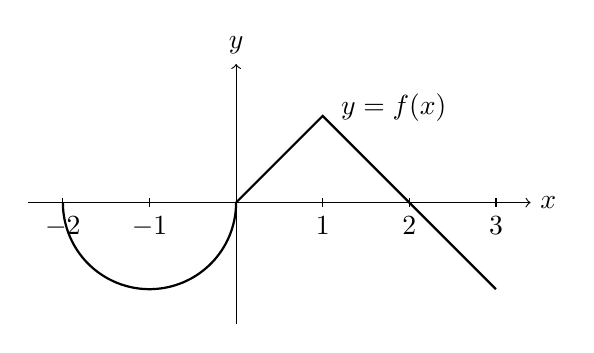
\begin{tikzpicture}[scale=1.1]
\draw[->](-2.4,0)--(3.4,0) node[right]{$x$};
\draw[->](0,-1.4)--(0,1.6) node[above]{$y$};
\draw[thick,domain=180:360,samples=70] plot ({-1+cos(\x)},{sin(\x)});
\draw[thick](0,0)--(1,1)--(3,-1);
\foreach \x in {-2,-1,1,2,3}{\draw(\x,.05)--(\x,-.05) node[below]{$\x$};}
\node[right] at(1.1,1.1){$y=f(x)$};
\end{tikzpicture}
\end{center}
\textbf{词义。}inflection point：拐点，曲线凹凸性改变之处；不是极值点，也不要求二阶导数在该点存在。

\textbf{错因。}选C。不清楚 inflection point；还把 $f$ 的尖角或不可微误传给 $g$，但 $g$ 是 $f$ 的积分。应先写 $g'=f$、在可用处 $g''=f'$。

\textbf{解答。}$f$ 在 $-1$ 由减变增，在1由增变减，因此 $g$ 有两个拐点，$B=2$；0两侧 $f$ 都递增，不是拐点。$f$ 在整个区间连续，所以 $g$ 在内部处处可微，端点按题目通常的一侧约定，$C=0$。$g$ 在 $[-2,0]$ 递减，在 $[0,2]$ 递增，在 $[2,3]$ 递减；比较候选最大值 $g(-2)=\pi/2$ 与 $g(2)=1$，得 $A=\pi/2$。所以 $0<\pi/2<2$，选D。端点若坚持要求双侧定义，则原题需说明延拓，考试通常不据此计为不可微点。

\subsection{38. 子群阶的存在性：E}
\label{ms:q38}
\textbf{原题。}If $G$ is a group of order 60, then $G$ does not necessarily have a subgroup of order:

(A) $2$ \quad (B) $3$ \quad (C) $4$ \quad (D) $5$ \quad (E) $6$.

\textbf{词义。}does not necessarily：不保证，要求找出可能不存在者；不是断言所有60阶群都没有该子群。

\textbf{错因。}选C。把“子群阶整除群阶”的必要条件当成充分条件，认为2、3、4、5、6均整除60所以都应存在；不熟悉柯西与Sylow的存在性区别。

\textbf{逐项判断。}2、3、5为整除60的素数，柯西定理保证相应阶的元素与子群。$60=2^2\cdot15$，Sylow保证4阶子群。6不是素数幂，不能用这些结论保证，因此选E。

\textbf{反例证明6确实可能不存在。}取 $G=A_4\times C_5$，阶60。若 $H$ 阶6，投影到 $C_5$ 的像阶同时整除6和5，只能为1，故 $H\subseteq A_4\times\{e\}$。而 $A_4$ 没有6阶子群：若有，其指数2，故正规，得到到 $C_2$ 的满同态。每个3循环的像阶整除3和2，只能为单位元；3循环生成 $A_4$，所以同态只能平凡，矛盾。$A_4$ 的非单位元素是3循环与双换位，双换位也能写成两个3循环之积，例如 $(12)(34)=(132)(134)$（右边先作用）。考场先记 \hyperref[review:lagrange]{拉格朗日的方向}及柯西、Sylow，不必临时重造反例。

\subsection{47. 传递关系必须检查自环：D}
\label{ms:q47}
\textbf{原题。}The vertex-edge graph above depicts a relation $\sim$ on the set $S=\{a,b,c,d\}$. For any $x\in S$ and $y\in S$, an arrow drawn from $x$ to $y$ on the graph signifies that $x\sim y$. What is the minimum number of additional arrows that must be drawn so that the relation represented by the resulting vertex-edge graph is transitive?

(A) Two \quad (B) Three \quad (C) Four \quad (D) Five \quad (E) Seven.

\begin{center}
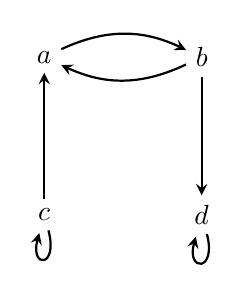
\begin{tikzpicture}[>=stealth]
\node(a)at(0,2){$a$};\node(b)at(2,2){$b$};\node(c)at(0,0){$c$};\node(d)at(2,0){$d$};
\path[->,thick](a)edge[bend left=25](b)(b)edge[bend left=25](a)(c)edge(a)(b)edge(d)(c)edge[loop below](c)(d)edge[loop below](d);
\end{tikzpicture}
\end{center}
\textbf{错因。}选A。复盘认为补 $a\to c,d\to b$ 两条就够，曾怀疑答案；但没有按有向传递性逐条检查，也漏掉 $a,b$ 必需的自环。图中原来是 $c\to a,b\to d$，不能把箭头当无向边。

\textbf{解答。}transitive：$x\sim y$ 且 $y\sim z$ 必须推出 $x\sim z$，允许 $x=z$。原有 $a\to b\to a$ 强制 $a\to a$，$b\to a\to b$ 强制 $b\to b$；$a\to b\to d$ 强制 $a\to d$；$c\to a\to b$ 强制 $c\to b$，再由 $c\to b\to d$ 强制 $c\to d$。这五条各自都必需，补完后 $a,b$ 各可到 $a,b,d$，$c$ 可到所有点，$d$ 只能到自身，已经传递，因此最少5条。新增箭头可能引出新的传递要求，不能补两条后只检查原来的路径。

\subsection{50. 正弦积分的级数估算：E}
\label{ms:q50}
\textbf{原题。}Estimate $\displaystyle\int_0^1\frac{\sin t}{t}\,dt$ to the nearest thousandth.

(A) $0.942$ \quad (B) $0.943$ \quad (C) $0.944$ \quad (D) $0.945$ \quad (E) $0.946$.

\textbf{词义。}nearest thousandth：四舍五入到小数点后三位。

\textbf{错因。}选C。知道用 Taylor 展开积分，但加减号写反，且 $1/18$ 的小数计算错误；方法正确，数值执行失误。复盘不应再把它记成“不会积分”。

\textbf{解答。}
\[
\frac{\sin t}{t}=1-\frac{t^2}{3!}+\frac{t^4}{5!}-\cdots,\qquad
I=1-\frac1{18}+\frac1{600}-\frac1{35280}+\cdots.
\]
前三项为 $0.946111\ldots$，交错级数余项绝对值小于 $1/35280<0.000029$，因此 $0.946082<I<0.946112$，保留三位小数必为 $0.946$。逐项积分后既要除阶乘，还要除幂次加1；先写分数与符号再转小数。

\subsection{52. 一致连续与柯西列：原题措辞有缺陷}
\label{ms:q52}
\textbf{原题。}Let $f:(0,1)\to(0,\infty)$ be a uniformly continuous function. Which of the following statements are true?
\begin{enumerate}[label=\Roman*.]
\item If $\{x_n\}$ is a Cauchy sequence in $(0,1)$, then $\{f(x_n)\}$ is a Cauchy sequence in $(0,\infty)$.
\item If $\lim_{n\to\infty}x_n$ exists, then $\lim_{n\to\infty}f(x_n)=f(\lim_{n\to\infty}x_n)$.
\item If $\{x_n\}$ and $\{y_n\}$ are two Cauchy sequences in $(0,1)$, then $\{|f(x_n)-f(y_n)|\}$ is a Cauchy sequence in $(0,\infty)$.
\end{enumerate}
(A) I only \quad (B) I and II only \quad (C) I and III only \quad (D) II and III only \quad (E) I, II, and III.

\textbf{作答与疑问。}选E，与答案表一致，但依据主要是“一致连续很强”的直觉，不会完整证明。审核发现II遗漏极限在定义域内的条件，III又把可能等于0的数列写成位于正数集；不能把原题E当作严格正确结论。

\textbf{定义与I。}uniformly continuous：对每个 $\varepsilon>0$，存在一个对所有输入点都有效的 $\delta>0$，使 $|x-y|<\delta\Rightarrow|f(x)-f(y)|<\varepsilon$。Cauchy sequence：尾部任意两项可彼此任意接近，不要求极限属于当前空间。给定 $\varepsilon$，由一致连续取 $\delta$，由输入列是柯西列取 $N$，使 $m,n>N$ 时 $|x_m-x_n|<\delta$，于是 $|f(x_m)-f(x_n)|<\varepsilon$，I正确。即使像列趋向0而0不在目标空间，它仍可在该空间中是柯西列。

\textbf{II的缺口。}取 $f(x)=x$、$x_n=1/(n+1)$，函数一致连续且映入正数，但极限为0，$f(0)$ 未定义。若补充 $\lim x_n=L\in(0,1)$，则由普通连续性已可推出等式，不需要一致连续。一致连续还保证可唯一连续延拓为实值函数 $\bar f$ 到 $[0,1]$，但原题未定义该延拓；延拓的端点值也可能为0，未必仍落在 $(0,\infty)$。

\textbf{III的正确核心与错误措辞。}由I，两像列是实数柯西列，且
\[
\big||f(x_m)-f(y_m)|-|f(x_n)-f(y_n)|\big|
\le |f(x_m)-f(x_n)|+|f(y_m)-f(y_n)|,
\]
所以绝对差列在 $\mathbb R$ 中是柯西列。但若 $x_n=y_n$，该列恒为0，不在原文的 $(0,\infty)$ 中。严格按题面仅I成立，对应A；若只把III改成“in $\mathbb R$”，则为C；同时补II的域内极限条件后才为E。复习应掌握证明与定义域限制，不必花时间猜作者意图。

\subsection{53. 正切函数的留数：B}
\label{ms:q53}
\textbf{原题。}Calculate $\displaystyle\frac1{2\pi i}\oint_C\tan z\,dz$, where $C$ is the circle $|z-1|=1$ parametrized counterclockwise.

(A) $-2$ \quad (B) $-1$ \quad (C) $0$ \quad (D) $1$ \quad (E) $2$.

\textbf{错因。}选D。已经尝试留数定理，但结果为正1；从计算可定位关键负号来自 $(\cos z)'=-\sin z$，不能把简单零点的导数比例漏掉。后续对话还暴露“二阶、三阶项积分为零”和高阶极点求导公式之间的混淆，已在 \hyperref[review:residues]{前置复变复习}完整说明。

\textbf{解答。}$\tan z=\sin z/\cos z$ 的极点是 $\pi/2+k\pi$。圆心1、半径1，只包含 $\pi/2$；$-\pi/2$、$3\pi/2$ 都在圆外。该点为简单极点，
\[
\operatorname{Res}(\tan z,\pi/2)
=\frac{\sin(\pi/2)}{-\sin(\pi/2)}=-1.
\]
逆时针积分是 $-2\pi i$，再除 $2\pi i$ 得 $-1$。公式不是把 $z-a$ 取为1，而是提取负一次项；分母的一阶 Taylor 系数为 $Q'(a)$，故要除以它。

\subsection{54. $A^3=A$：逐项反例与必然结论：D（实际答对）}
\label{ms:q54}
\textbf{原题。}Suppose $A$ is a $3\times3$ matrix with the property that $A^3=A$. Which of the following must be true?
\begin{enumerate}[label=(\Alph*)]
\item The eigenvalues of $A$ are distinct.
\item If $A$ is invertible, then $A^T=A$.
\item $A^2$ is the identity matrix or the zero matrix.
\item The trace of $A^2$ equals the rank of $A$.
\item The absolute value of the trace of $A^3$ equals the rank of $A$.
\end{enumerate}
\textbf{词义与作答。}must be true：对满足条件的所有矩阵成立；distinct：互不相同；trace：迹，对角元之和；rank：秩；transpose $A^T$：转置。原始蓝笔漏写最终字母，现明确实际选D，正确；仍收录所有选项以通过反例巩固。

\textbf{先取结构。}按通常实数或复数矩阵理解，$A$ 满足 $A(A-I)(A+I)=0$，其最小多项式整除无重根多项式 $t(t-1)(t+1)$，因此可对角化。特征值只能是 $0,1,-1$，但可以重复。设它们的重数为 $n_0,n_+,n_-$，则
\[
n_0+n_++n_-=3,\quad
\operatorname{rank}A=n_++n_-,\quad
\operatorname{tr}(A^2)=n_++n_-,\quad
\operatorname{tr}(A^3)=n_+-n_-.
\]
不是“特征值只有三个可能值”就自动可对角化；真正理由是湮灭多项式无重根。也可不靠对角化证明D：令 $P=A^2$，由 $A^4=A^2$ 得 $P^2=P$，幂等矩阵的迹等于秩；又 $\ker A=\ker A^2$，因为 $A^2v=0\Rightarrow Av=A^3v=A(A^2v)=0$，故两者秩相等。

\textbf{A不必真。}取 $A=I_3$，满足 $A^3=A$，三个特征值均为1，并不互异。不要把“最小多项式无重根”误解成“特征多项式无重根”。

\textbf{B不必真。}可逆只推出 $A^2=I$，不推出对称。反例
\[
A=\begin{pmatrix}1&1&0\\0&-1&0\\0&0&1\end{pmatrix}.
\]
直接相乘 $A^2=I_3$，故可逆且 $A^3=A$，但 $A^T\ne A$。可对角化也不等于能用正交矩阵对角化；实对称是更强性质。

\textbf{C不必真。}取 $A=\operatorname{diag}(1,0,0)$，则 $A^3=A$，但 $A^2=A$ 既非单位矩阵也非零矩阵。

\textbf{D必真。}由上述重数计数，平方把 $1,-1$ 都变成1，0仍为0，所以 $\operatorname{tr}(A^2)=n_++n_-=\operatorname{rank}A$。只有这一项对所有情况成立。

\textbf{E不必真。}取 $A=\operatorname{diag}(1,-1,0)$，满足条件，但 $|\operatorname{tr}(A^3)|=0$，$\operatorname{rank}A=2$。迹允许正负抵消，秩不会抵消。一般 $|n_+-n_-|\le n_++n_-$，仅在非零特征值不同时含正负两类时相等。

\subsection{55. 四次多项式用有限差分：A}
\label{ms:q55}
\textbf{原题。}Selected values of a polynomial $f(x)$ of degree 4 are given in the table above. What is the value of $f(5)$?
\[
\begin{array}{c|rrrrr}x&0&1&2&3&4\\\hline f(x)&1&-5&-7&-2&3\end{array}
\]
(A) $-9$ \quad (B) $-4$ \quad (C) $2$ \quad (D) $7$ \quad (E) $11$.

\textbf{错因。}选E。以为必须求四次多项式全部系数，解线性方程组甚至求逆，估计超过五分钟，因而放弃猜选。主要缺少有限差分方法，不是题目必然计算量大。即使走系数法也不必求逆，但本题有更直接结构。

\textbf{解答。}等距节点下，次数4的多项式四阶差分恒定；因为 $\Delta p(x)=p(x+1)-p(x)$ 每作用一次降一次次数。列出
\[
\begin{array}{c|rrrrr}
f&1&-5&-7&-2&3\\
\Delta f&-6&-2&5&5\\
\Delta^2f&4&7&0\\
\Delta^3f&3&-7\\
\Delta^4f&-10
\end{array}
\]
向右延续第四阶 $-10$，依次回加：下一三阶为 $-17$，二阶为 $-17$，一阶为 $-12$，所以 $f(5)=3-12=-9$。也可直接用 $\Delta^5 f(0)=0$：
\[
f(5)=5f(4)-10f(3)+10f(2)-5f(1)+f(0)=-9.
\]
考试优先画差分表，少背易错的正负系数。

\subsection{56. 解析函数模长恒定：A（猜对后巩固）}
\label{ms:q56}
\textbf{原题。}Let $g(z)$ be an analytic function such that $|g(z)|=3$ for all $z$ in the open disk $|z|<2$. If $g(1)=3i$, find all possible values of $g(-1)$.

(A) $\{3i\}$ \quad (B) $\{-3i\}$ \quad (C) $\{3i,-3i\}$ \quad (D) $\{3,-3,3i,-3i\}$ \quad (E) $\{z\in\mathbb C:|z|=3\}$.

\textbf{作答记录。}选A正确，但自述蒙对，只记得可能有“模长恒定则常值”。需要补齐解析性、连通开区域以及“整个区域内”的条件。

\textbf{解答。}圆盘连通，若 $g$ 非常值，开映射定理要求其像在复平面中开，但 $|g|=3$ 的像落在圆周上，不含任何开圆盘，矛盾。因此 $g$ 常值，由 $g(1)=3i$ 得 $g(-1)=3i$，只有A正确。也可用CR：$g=u+iv$，$u^2+v^2=9$ 求偏导，代入CR得
\[
u u_x+v v_x=0,\qquad -u v_x+v u_x=0.
\]
系数矩阵行列式绝对值为 $u^2+v^2=9$，故 $u_x=v_x=0$，再由CR得其他偏导为0，所以常值。反例边界：$e^{it}$ 作为实参数曲线模长恒定但不恒定；$g(z)=z$ 在单位圆边界模长恒定但在圆盘内不恒定。不要遗漏假设。

\subsection{57. 螺线闭包连通但不道路连通：C}
\label{ms:q57}
\textbf{原题。}Let $C_1$ be the curve defined by the polar equation $r=\theta/(\theta+1)$ for $\theta\ge0$, and let $C_2$ be the circle defined by $x^2+y^2=1$. Let $C=C_1\cup C_2$. Which of the following statements are true with respect to the standard topology on $\mathbb R^2$?
\begin{enumerate}[label=\Roman*.]
\item For any point $P\in C$, there exists an open disk centered at $P$ containing some point $Q\in C$ such that $P\ne Q$.
\item For any collection $\mathcal F$ of open disks such that $C\subseteq\bigcup\mathcal F$, there exists a finite subcollection $\mathcal G\subseteq\mathcal F$ such that $C\subseteq\bigcup\mathcal G$.
\item For any pair of points $P\in C$ and $Q\in C$, there exists a continuous function $f:[0,1]\to C$ such that $f(0)=P$ and $f(1)=Q$.
\end{enumerate}
(A) I only \quad (B) II only \quad (C) I and II only \quad (D) II and III only \quad (E) I, II, and III.

\textbf{错因。}选E。I、II判断正确，但不熟悉III所表达的道路连通；复盘时提出“可能连通但非道路连通”的直觉，正是正确区别。不是没有看出螺线趋向圆，而是不清楚趋近是否足以构造连续路径。

\textbf{I真。}更强的说法“每个开邻域都含别的集合内点”也成立：圆周点沿圆即可找到邻近点，螺线点沿连续参数微移即可。原题只写存在一个开圆盘，逻辑上更弱，并不恰好等同无孤立点；本集合满足更强版本，结论不受影响。

\textbf{II真。}这是以开圆盘为基的紧性表述。$C$ 有界且闭：螺线的有界参数序列极限仍在螺线上，无界参数子列的半径趋1，极限在单位圆；反过来每个圆周点可沿固定角加 $2k\pi$ 得到螺线点趋向它。因此 $C=\overline{C_1}$，由欧氏空间闭且有界判据紧。

\textbf{III假。}道路连通要求一条有限参数区间上的连续路径真正连接两点，单纯无限接近不够。假设从螺线非圆周点到圆周存在路径 $\gamma$，令 $t_0$ 是首次碰到圆周的时刻。对 $t<t_0$，路径在螺线上；半径 $\rho(t)$ 决定唯一螺线参数 $\theta(t)=\rho(t)/(1-\rho(t))$。当 $t\uparrow t_0$，$\rho(t)\to1$，所以 $\theta(t)\to\infty$。令 $\gamma(t_0)$ 的辐角为 $\phi$，连续且趋于无穷的 $\theta(t)$ 在靠近 $t_0$ 时必依次经过 $\phi+2k\pi$ 与 $\phi+(2k+1)\pi$，对应位置分别趋向圆上的相反两点，不能都趋于 $\gamma(t_0)$，矛盾。故只I、II真，选C。$C_1$ 是区间连续像，连通；闭包 $C$ 仍连通，所以此例确实连通但非道路连通。

\subsection{61. 复指数函数之间的线性关系：B}
\label{ms:q61}
\textbf{原题。}Let $V$ be the vector space of continuous functions $\mathbb C\to\mathbb C$ under pointwise addition and scalar multiplication by complex numbers, and let $A$ be the set of fourth roots of unity in the complex plane. For each $\alpha\in A$, define the set $S_\alpha=\{\cos\alpha z,\sin\alpha z,e^{\alpha z}\}$. What is the dimension of the subspace of $V$ spanned by $\bigcup_{\alpha\in A}S_\alpha$?

(A) $3$ \quad (B) $4$ \quad (C) $6$ \quad (D) $8$ \quad (E) $12$.

\textbf{错因。}选C。列出 $\cos z,\sin z,e^z,e^{-z},e^{iz},e^{-iz}$ 六个生成函数，就把生成集当成基；复盘怀疑它们线性相关，确实如此。这里允许复数系数，不只实数系数。

\textbf{解答。}$A=\{1,-1,i,-i\}$。欧拉公式给出
\[
e^{iz}=\cos z+i\sin z,\quad e^{-iz}=\cos z-i\sin z,\quad
\cos z=\frac{e^{iz}+e^{-iz}}2,\quad
\sin z=\frac{e^{iz}-e^{-iz}}{2i}.
\]
$\cos(iz)=(e^z+e^{-z})/2$，$\sin(iz)=(e^{-z}-e^z)/(2i)$。因此全部函数由四个指数 $e^z,e^{-z},e^{iz},e^{-iz}$ 张成。它们线性无关：若 $\sum_{j=1}^4 c_je^{\lambda_jz}=0$，在0处求0至3阶导得 $\sum c_j\lambda_j^k=0$，$k=0,1,2,3$；$\lambda_j=1,-1,i,-i$ 互异，范德蒙德矩阵行列式 $\prod_{j<k}(\lambda_k-\lambda_j)\ne0$，故全为零。维数恰为4，选B。只证能由四个张成得到的是维数至多4，还需独立性确认恰好4。

\subsection{62. 所有方向导数存在不等于可微：原答案A错误}
\label{ms:q62}
\textbf{原题。}Which of the following must be true of a function $f:\mathbb R^2\to\mathbb R$?
\begin{enumerate}[label=\Roman*.]
\item If $\partial f/\partial x$ and $\partial f/\partial y$ exist and are continuous at $(0,0)$, then $f$ is differentiable there.
\item If $f$ has directional derivatives in all directions at $(0,0)$, then $f$ is differentiable there.
\item If $\partial^2f/\partial x\partial y$ and $\partial^2f/\partial y\partial x$ exist at $(0,0)$, then they are equal there.
\end{enumerate}
(A) None \quad (B) II only \quad (C) I and II only \quad (D) I and III only \quad (E) II and III only.

\textbf{错因与勘误。}选B，原先排除I、III后对II犹豫而猜选；这是对方向导数与全微分关系不清，不只是“二选一运气不好”。但答案表A同样错误：按通常“偏导数在邻域存在并在原点连续”的含义，I是标准充分条件，正确组合是 I only，而选项缺少它。作者解答用 $xy/(x^2+y^2)$ 在原点补0反驳I，但该例 $f_x(0,y)=1/y$（$y\ne0$），偏导数在原点不连续，未满足前提，反例无效。来源：\url{https://www.mathsub.com/wp-content/uploads/mathsub-test-01-solutions.pdf}。

\textbf{I为什么真。}设 $f_x(0,0)=a,f_y(0,0)=b$，把增量拆成
\[
f(h,k)-f(0,0)=[f(h,k)-f(0,k)]+[f(0,k)-f(0,0)].
\]
沿水平与竖直线分别用一元中值定理，得到 $f_x(\xi,k)h+f_y(0,\eta)k$，其中 $\xi$ 介于0与 $h$、$\eta$ 介于0与 $k$。偏导在原点连续，减去 $ah+bk$ 后是 $o(\sqrt{h^2+k^2})$，正是可微。零增量分支直接处理即可。

\textbf{II反例：连续、所有方向导数存在，仍不可微。}取
\[
f(x,y)=\begin{cases}x^3/(x^2+y^2),&(x,y)\ne(0,0),\\0,&(x,y)=(0,0).\end{cases}
\]
由 $|f(x,y)|\le|x|\le\sqrt{x^2+y^2}$，原点连续。对任意非零向量 $v=(a,b)$，
\[
D_vf(0,0)=\lim_{t\to0}\frac{f(ta,tb)}t=\frac{a^3}{a^2+b^2},
\]
所以不仅两个坐标方向，所有方向导数均存在。但 $f_x(0,0)=1,f_y(0,0)=0$，若可微，唯一可能的线性近似为 $L(h,k)=h$。沿 $h=k=t>0$，
\[
\frac{f(t,t)-L(t,t)}{\sqrt{t^2+t^2}}=-\frac1{2\sqrt2}\not\to0.
\]
故不可微。等价地，可微强制 $D_vf=L(v)$ 关于方向向量线性，而上式不线性；取单位对角方向时，实际方向导数为 $1/(2\sqrt2)$，线性近似却要求 $1/\sqrt2$。不是“已经可微但不满足线性”，而是反证：若可微必须线性，实际不线性，所以不可微。反向也要谨慎：所有方向导数存在且形成线性映射，本身仍不能替代统一的全微分余项估计。

\textbf{III反例。}取
\[
F(x,y)=\begin{cases}xy(x^2-y^2)/(x^2+y^2),&(x,y)\ne(0,0),\\0,&(x,y)=(0,0).\end{cases}
\]
直接按定义得 $F_x(0,y)=-y$、$F_y(x,0)=x$，所以 $\partial_y(\partial_xF)(0,0)=-1$，而 $\partial_x(\partial_yF)(0,0)=1$。混合偏导仅存在不保证相等；常用充分条件是它们在邻域连续。记住正确关系：偏导连续足以可微，可微推出连续及各方向导数由同一线性映射给出；连续加所有方向导数存在仍不足。

\subsection{64. 理想乘积、交与和：D}
\label{ms:q64}
\textbf{原题。}Let $A$ and $B$ be ideals of a ring $R$, and define the ideals $A+B$ and $AB$ as follows:
\[
A+B=\{a+b:a\in A,b\in B\},\qquad
AB=\{a_1b_1+\cdots+a_nb_n:a_i\in A,b_i\in B,\ i\in\{1,\ldots,n\}\},\quad n\in\{1,2,\ldots\}.
\]
Which of the following correctly orders $A+B$, $AB$, and $A\cap B$ via inclusion?

(A) $AB\subseteq A+B\subseteq A\cap B$ \quad
(B) $A\cap B\subseteq AB\subseteq A+B$ \quad
(C) $A\cap B\subseteq A+B\subseteq AB$ \quad
(D) $AB\subseteq A\cap B\subseteq A+B$ \quad
(E) $A+B\subseteq A\cap B\subseteq AB$.

\textbf{错因。}选C。第一步 $A\cap B\subseteq A+B$ 的证明正确：$x=x+0$ 且理想包含0。错误在试图用 $a+b=a\cdot1+1\cdot b$ 证明 $A+B\subseteq AB$；这需要第一个1在B、第二个1在A，但理想不一定含1。含1的理想其实只能是全环。

\textbf{解答。}对每项 $a_ib_i$，A的右吸收性使其在A，B的左吸收性使其在B；两理想对加法封闭，故有限和也在交中。再用 $x=x+0$ 得
\[
\boxed{AB\subseteq A\cap B\subseteq A+B}.
\]
选D。取 $R=\mathbb Z,A=4\mathbb Z,B=6\mathbb Z$，则 $AB=24\mathbb Z$、$A\cap B=12\mathbb Z$、$A+B=2\mathbb Z$，两个包含均严格；这个例子也逐一排除其余排序。理想乘积允许有限和，与 Practice 1 的50题单个乘积集合不同。

\subsection{65. 等差数列拓扑：E（时间不足猜选，低优先级）}
\label{ms:q65}
\textbf{原题。}For each pair of integers $a$ and $b$, let the set $\{a+bn:n\in\mathbb Z\}$ be denoted $a+b\mathbb Z$. Consider the topology $\mathcal T$ on $\mathbb Z$ whose basis is $\{a+b\mathbb Z:a,b\in\mathbb Z\text{ and }b\ne0\}$. Which of the following statements is false?
\begin{enumerate}[label=(\Alph*)]
\item $(\mathbb Z,\mathcal T)$ is Hausdorff.
\item $(\mathbb Z,\mathcal T)$ is totally disconnected.
\item The set $\{0\}$ is closed under $\mathcal T$.
\item No nonempty open sets of $\mathcal T$ are finite.
\item Exactly two sets of $\mathcal T$ are both open and closed.
\end{enumerate}
\textbf{作答与复习取舍。}选C；后段时间不足而猜选，且不愿在现阶段深入这种陌生拓扑。保留最短反例与必要定义，不当成单纯粗心。

\textbf{最短解。}basis：基，任意开集是基本开集的并。偶数集 $2\mathbb Z$ 是基本开集，其补集奇数集 $1+2\mathbb Z$ 也开，所以偶数集既开又闭，且非空非全集。除空集、全集外已有第三个既开又闭集合，故E假，选E；无需先证明所有其他项。

\textbf{A真。}Hausdorff要求不同点有不交开邻域。给定整数 $x\ne y$，取正整数 $n>|x-y|$，则 $x+n\mathbb Z$、$y+n\mathbb Z$ 不相交，否则 $n\mid x-y$，矛盾。

\textbf{B真。}totally disconnected：每个连通子集至多一个点。任意含 $x\ne y$ 的子集S，用上面的同余类 $U=x+n\mathbb Z$ 及补集分开；补集是其他有限个模 $n$ 同余类之并，开。$U\cap S$ 与 $(\mathbb Z\setminus U)\cap S$ 是不交非空相对开集，故S不连通。

\textbf{C真。}对任意非零整数 $x$，取 $n>|x|$，则 $x+n\mathbb Z$ 包含x但不含0，故 $\mathbb Z\setminus\{0\}$ 是开集，单点集闭；它不必开。

\textbf{D真。}非空开集中的任一点都有包含于该开集的基本开邻域，而每个 $a+b\mathbb Z$（$b\ne0$）都是无限集，故非空开集无限。不必分析任意无穷交，拓扑只要求有限交保持开。

\subsection{66. 模与极小生成集：B（时间不足猜选，低优先级）}
\label{ms:q66}
\textbf{原题。}Let an abelian group $M$ form a left module over a ring $R$. We say that a subset $S$ of $M$ is a spanning set of $M$ if for every $m\in M$, there exist $\{r_1,\ldots,r_n\}\subseteq R$ and $\{s_1,\ldots,s_n\}\subseteq S$ such that $m=\sum_{i=1}^n r_is_i$.

We call this spanning set $S$ minimal if no proper subset of $S$ is a spanning set for $S$. In addition, $S$ is called a basis for $M$ if $m=0$ implies $r_1=r_2=\cdots=r_n=0$.

Which of the following statements must be true?
\begin{enumerate}[label=\Roman*.]
\item If $R$ is finite, then any basis $S$ of $M$ is finite.
\item If $S$ and $S'$ are two distinct minimal spanning sets of $M$, then $|S|=|S'|$.
\item If $R$ is a field and $S$ is a finite minimal spanning set of $M$, then $S$ is a basis of $M$.
\end{enumerate}
(A) II only \quad (B) III only \quad (C) I and II only \quad (D) I and III only \quad (E) II and III only.

\textbf{题面说明。}原文“a spanning set for $S$”按上下文应指生成 $M$；基的线性无关条件按有限个互异生成元、任意线性组合理解。以上保留原题措辞，解答使用标准定义。

\textbf{错因与定位。}选C；时间不足猜选，又不熟悉环上的模、minimal与minimum的区别。当前不优先深入模论，但可用整数例子理解本题。

\textbf{基础概念。}left module：左模，类似向量空间，但系数取自环，数乘满足加法分配及 $(rs)m=r(sm)$，通常还要求 $1m=m$；环中非零系数可能不可逆。spanning set：生成集，每个元素为有限线性组合；minimal：不能删除任何元素后仍生成，并非元素数量全局最少的 minimum；basis：生成且线性无关。一般模不一定有基，不应把向量空间结论全部照搬。

\textbf{I假：有限系数集不限制基的大小。}取 $R=\mathbb F_2$、$M=\mathbb F_2[x]$，作为域 $\mathbb F_2$ 上的向量空间，基为 $\{1,x,x^2,\ldots\}$，无限；每个多项式仍只用有限多个基向量。系数只有0、1不代表只有有限个独立方向。

\textbf{II假：最简单的整数反例。}取 $R=M=\mathbb Z$，允许整数线性组合。$\{1\}$ 生成所有整数且不能删；$\{2,3\}$ 也生成，因为 $1=3-2$，而只留2或只留3分别仅生成 $2\mathbb Z$、$3\mathbb Z$，所以它也极小。两组大小为1、2，II不成立。$\{2,3\}$ 并非基：$3\cdot2-2\cdot3=0$ 是非平凡整数线性关系，但不能除以3或2把另一元素表示成整数倍。

\textbf{III真：域上的有限极小生成集就是基。}若 $S=\{v_1,\ldots,v_n\}$ 线性相关，有 $\sum a_iv_i=0$ 且某系数 $a_j\ne0$。域中 $a_j$ 可逆，故 $v_j=-\sum_{i\ne j}(a_i/a_j)v_i$，删掉 $v_j$ 仍能生成，违反极小性。因此线性无关，故为基。关键不是“有限”本身，而是可以除以非零系数。只有III真，选B。

\subsection{本套错因与下一次检查动作}
\label{ms:summary}
\begin{itemize}
\item 审题：12把“第五次才达第三次成功”读成前五次成功数；14漏上下限相同；35漏整数条件；最后分别写清事件、特殊端点、变量取值范围。
\item 算术及代入：13半径／直径与根式因子2；27指数 $xy$ 在给定点为0；50符号及 $1/18$；53分母求导漏负号。执行时保留分数，代入后先简化复合量，再检查符号。
\item 方法缺口：31用复奇点距离代替求系数；55用有限差分代替解方程组。这两题不应继续列为必然耗时超过五分钟的题。
\item 概念：24区分 unit/unity；25指数实部决定包络而虚部带来振荡；36先写 $g'=f$；38不能倒用拉格朗日；47检查自环与新增路径；61生成集不一定独立；64理想不一定含1。
\item 答对仍需巩固：52补一致连续到柯西列的证明并标勘误；54实际选D正确，但逐项反例要会；56补解析函数常模的条件。
\item 题目质量：62按通常数学定义I真、II与III假，选项缺 I only；52按严格原文也不能选E。不要用错误答案破坏正确知识。
\item 取舍：65、66按现阶段策略低优先级，保留短解和基本反例；不把“复盘后能懂”直接当作下一次一定能在时限内独立做对。
\end{itemize}

\end{document}

